\chapter{Deep integrations on polarization with PAPER-128}
\label{chapter:eor_window_psa128}

In Chapter~\ref{chapter:eor_window_paper32img}, I presented polarized power spectra from a short integration -- a few hours of one night -- over a wide range of $k_{\perp}$-modes probed by the PAPER-32 polarized imaging array \citep{Kohn.16}. Chapter~\ref{chapter:eor_window_HERA} presented the first power spectral results from HERA. The HERA-19 commissioning array was small and dense, meaning that only a few $k_{\perp}$-modes were accessible. For that study, we averaged over 10 hours per night, for 8 consecutive nights \citep{Kohn.18}. This Chapter presents results from the PAPER-128 array. In this Chapter I present roughly one quarter of the total number of observations recorded by this interferometer (Section~\ref{sec:psa128_obs}). I show results of a deep integration on a very narrow range of $k_{\perp}$-modes (corresponding to $\sim$30\,m spacings of the redundant grid; Section~\ref{sec:psa128_results}) and discuss the implications for deep, fully-polarized integrations with large interferometers (Section~\ref{sec:psa128_conc}).

\section{Observations \& Reduction}
\label{sec:psa128_obs}
 
PAPER-128 was the largest build-out of the PAPER experiment. As described in Chapter~\ref{chapter:instruments},  PAPER-128 consisted of 128 antennas, 112 of which were arranged in a redundant grid. An annotated photograph of the array is shown in Figure~\ref{fig:psa128photo}. In this section, I review the PAPER-128 campaign (Section~\ref{subsec:psa128_obs_overview}) and the subsequent reduction of roughly one quarter of the total number of observations (Section~\ref{subsec:psa128_s1e2_reduction}).

\begin{figure}
\includegraphics[width=0.8\textwidth, angle=270]{chapters/psa128_pol/figures/array_photo_diagram.pdf}
\caption[An annotated photograph of the PAPER-128 array.]{An annotated photograph of the PAPER-128 array, looking to the East. Highlighted are the 112 antenna redundant grid, with 15\,m East-West spacings between each row; outlier antennas from the main grid used to increase \textit{uv}-coverage; coaxial cables running to the receiverators and correlator (see Chapter~\ref{chapter:instruments}). An inset panel shows a PAPER sleeved dipole. Photo credit: J. E. Aguirre. Figure credit: C. D. Nunhokee; \citep{Nunhokee_thesis}.}
\label{fig:psa128photo}
\end{figure}

\subsection{Overview of PAPER-128 observations}
\label{subsec:psa128_obs_overview}
Observations were recorded for two years, with first light on November 20th 2013 and final readings on January 27th 2015. However, these observations were not always contiguous. Human errors, experimentation and malfunctioning electronics required the correlator and connected electronics to be turned off and restarted, altering the characteristic phasing and gain scale of the array. Each of these restarts constituted the beginning of a new ``Epoch" of the array which required different quality assurance steps and initial calibration stages. Table~\ref{tab:seasons_psa128} summarizes the length and nature of these Epochs. 

\begin{deluxetable}{lllll}
\centering
\label{tab:seasons_psa128}
\tablewidth{0pt}
\tablecaption{PAPER-128 Observing Seasons \& Epochs}
\tabletypesize{\footnotesize}
\tablehead{
\colhead{Season} & \colhead{Epoch} & \colhead{Julian Dates} & \colhead{Calendar Dates} & \colhead{Notes} \\
}
\startdata
1 & 1 & 2456617 - 2456673 & Nov 20, 2013 - Jan 15, 2014 & 1/8 F-Engine failure \\
   & 2 & 2456678 - 2456724 & Jan 20, 2014 - Mar 7, 2014 &  Good \\
2 & 1 & 2456625 - 2456732 & Mar 8, 2014 - Mar 7, 2014 & Too few data \\
   & 2 & 2456843 - 2456873 & Jul 4, 2014 - Aug 3, 2014 & Uninteresting LST range \\
   & 3 & 2456881 - 2456928 & Aug 11, 2014 - Sep 27, 2014 &  Many malfunctioning antennas \\
   & 4 & 2456942 - 2457008 & Oct 11, 2014 - Dec 11, 2014 &  Good \\
   & 5 & 2457030 - 2457050 & Jan 7, 2015 - Jan 27, 2015 &  Many malfunctioning antennas\\
\enddata
\end{deluxetable}

Figure~\ref{fig:psa128_epochs} illustrates the challenge imposed by the correlator restarts. Epoch changes were characterized by large shifts in the overall phase of visibilities, of course leading to changed magnitudes of the real and imaginary parts of the visibilities recorded. The quality assurance metrics described in Chapter~\ref{chapter:data_prep_and_proc} were sensitive to these changes. Of course, absolute calibration -- that is phasing to the correct point on the sky and scaling the visibilities from arbitrary to physical flux density units -- had to be run separately on individual Epochs.

\begin{figure}
\centering
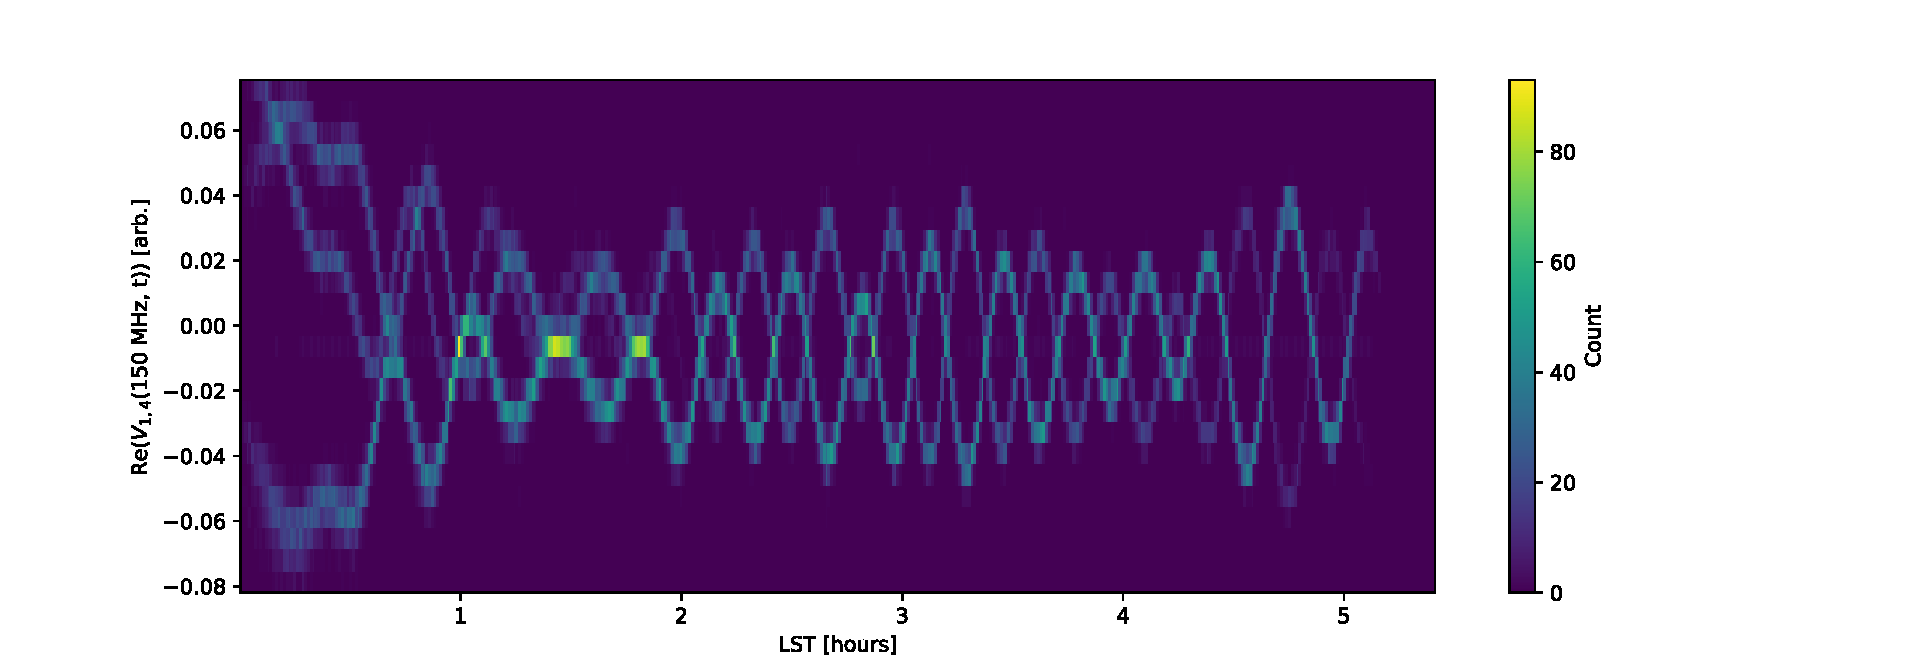
\includegraphics[width=0.7\textwidth]{chapters/psa128_pol/figures/S2_chan100_hist.pdf}
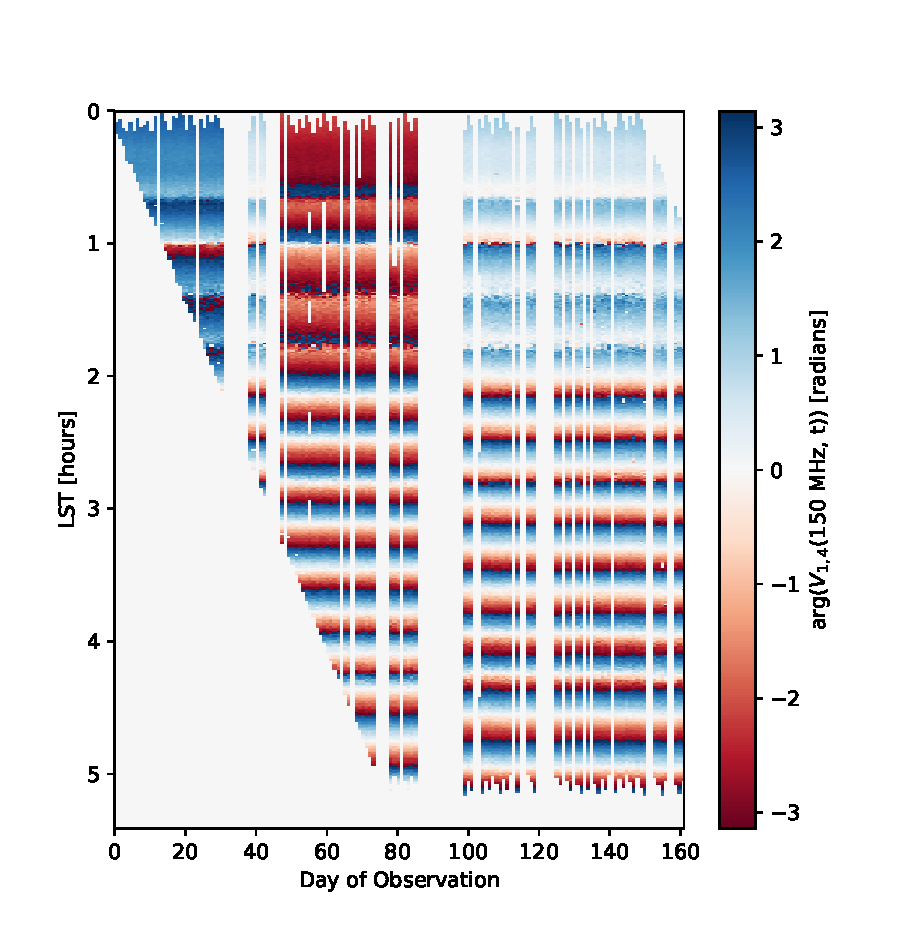
\includegraphics[width=0.5\textwidth]{chapters/psa128_pol/figures/S2_chan100_phasegrid.pdf}
\caption[The challenge of Epoch changes.]{The challenge of Epoch changes. Shown are all of the Season 2 time samples of the visibilities recorded by the 30\,m baseline between antennas 1 and 4, LSTs 0--5, for only the 150\,MHz frequency bin. The above panel shows a histogram of the real part of the visibilities as a function of LST -- there is a dramatic change in magnitude with respect to LST. Likewise, the lower panel shows the phase of each visibility sample (color axis) as a function of LST (vertical axis) and day of observation (x axis). There are obvious large shifts in phase, which require separate calibration stages.}
\label{fig:psa128_epochs}
\end{figure}

As shown in Table~\ref{tab:seasons_psa128}, Season 2 had a larger number of observed nights than Season 1. However, the analysis of Season 2 was especially challenging due to large numbers of malfunctioning antennas. This may have been due to the antennas ageing past a critical point. Nothing in the array was replaced during build-outs except for the correlator; 32 of the antennas had been out in the desert for 4--5 years (PAPER-32) and another 32 for 3--4 years (PAPER-64). Most of the time, these were the antennas that were identified as malfunctioning.

Season 2 Epoch 4 was relatively well-behaved, and may be analyzed in the future. For this work, we concentrated our analysis on Season 1. Season 1 Epoch 2 was ten days shorter than Season 1 Epoch 1, but Epoch 1 had two major challenges associated with it: a data loss event, and an F-engine failure. Due to human error, Epoch 1 data was deleted and had to be restored and recompressed (see Chapter~\ref{chapter:data_prep_and_proc}). This was almost entirely successful, at the loss of one week's worth of observations. The F-engine failure was more critical. We discovered during out analysis that exactly one eighth of the antennas in the array produced noise-like visibilities with the rest of the array, but normal correlations between one another. These antennas had ``seceded" from the array. They shared the characteristic of all being attached to the same F-engine (of which there were eight; see Figure~\ref{fig:instruments_PAPER_Signal_Chain}). This suggested that there was a clock-offset on that F-engine, resulting in no correlation between the signal from those antennas and those running through the other in-sync F-engines.

This left Season 1 Epoch 2 as the most well-characterized and well-behaved Epoch of PAPER-128 observations, and we focused on this Epoch alone from now on. Cross-polarization metrics identified seven incorrectly-rotated antennas, which were corrected during initial processing. Eight antennas were identified as malfunctioning by mean visibility amplitude metrics, including one of those that was incorrectly-rotated. The state of the array for Season 1 Epoch 2 is summarized in Figure~\ref{fig:s1e2_array}.

\begin{figure}
\centering
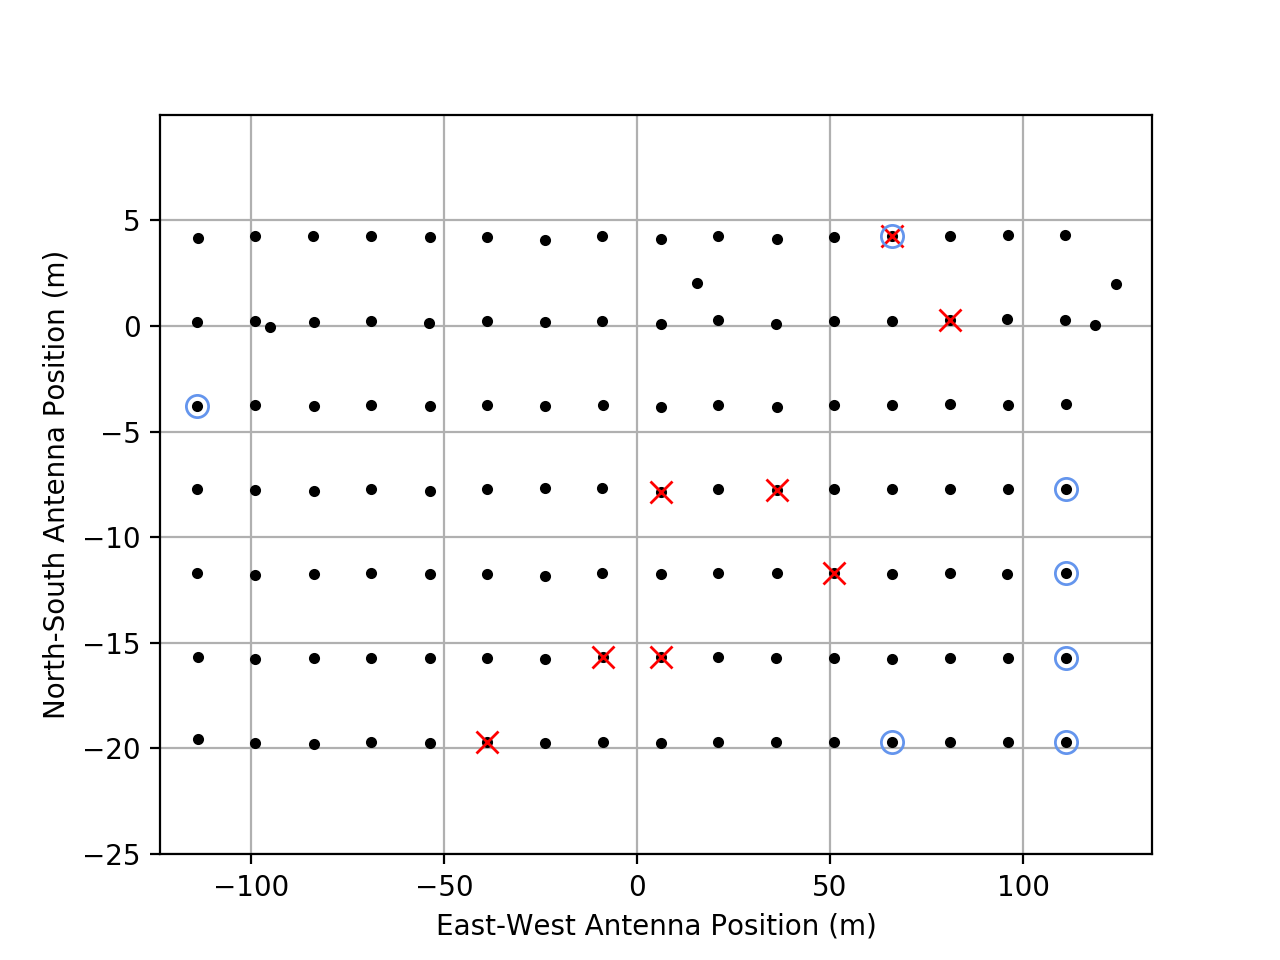
\includegraphics[width=0.6\textwidth]{chapters/psa128_pol/figures/s1e2_array.png}
\caption[Good, bad and rotated antennas in Season 1 Epoch 2.]{Good, bad (red crosses) and rotated (blue circles) antennas in Season 1 Epoch 2, as identified by the cross-polarization and visibility amplitude metrics defined in Chapter~\ref{chapter:data_prep_and_proc}.}
\label{fig:s1e2_array}
\end{figure}

\subsection{Reduction of Season 1 Epoch 2 data}
\label{subsec:psa128_s1e2_reduction}

After correcting for cross-polarized and malfunctioning antennas, we were able to begin processing the data using the redundant calibration techniques described in Chapter~\ref{chapter:polcal}. We used the phase-flattening algorithm described in Section~\ref{sec:polcal_data} to solve for phase slopes for each antenna. This was performed for the North-South and East-West feed arms separately using the linear instrumental polarizations (`nn' and `ee'), as this method is sensitive to signal-to-noise. We performed a single calculation of these overall delays at the start of the Epoch, and applied those to the rest of the days observed. These overall delays are largely due to electrical delays along the cables leading to the receiverators and the correlator, so we did not expect them to vary a by large amount.

\subsubsection{Redundant calibration}
\label{subsubsec:psa128_redcal}
After phase-wraps were flattened, the {\sc omnical} algorithm could be invoked safely. For this study, we implemented the \textit{4pol+minV} calibration method. For a full exploration of {\sc omnical}ibration methods, see Chapter~\ref{chapter:polcal}. Briefly, the \textit{4pol+minV} calibration scheme redundantly solves for diagonal gains for the North-South and East-West feed arms at the same time, \textit{and} imposes that the `ne' and `en' visibilities are equal. That is, it produces a redundant calibration which minimizes pseudo-Stokes V. Figures~\ref{fig:psa128_pre_post_abs} and \ref{fig:psa128_pre_post_phs} show the successful results of the \textit{4pol+minV} {\sc omnical}ibration, where visibilities from 30\,m East-West baselines showed a high degree of redundancy in all pseudo-Stokes polarizations, and pseudo-Stokes V is almost complete noise-like.

\begin{figure}
\centering
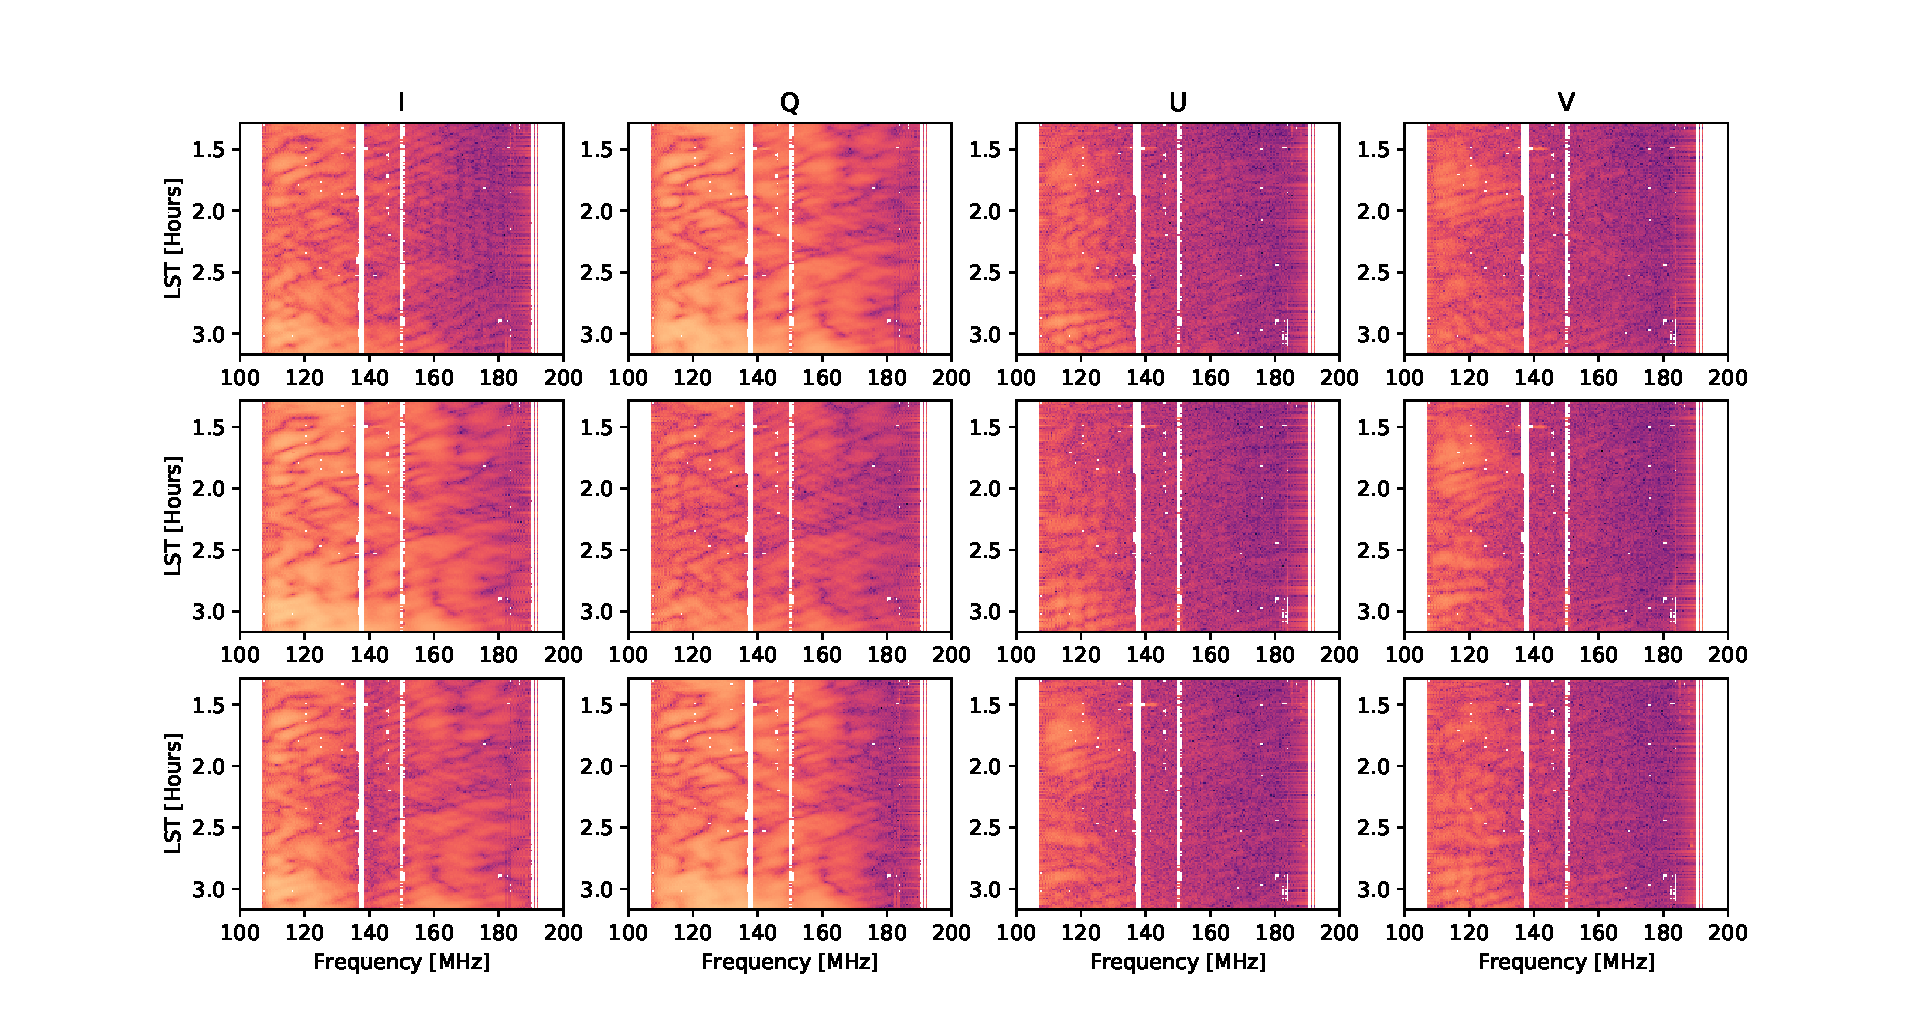
\includegraphics[width=0.8\textwidth]{chapters/psa128_pol/figures/nocal_IQUV_6680_0-5.pdf}
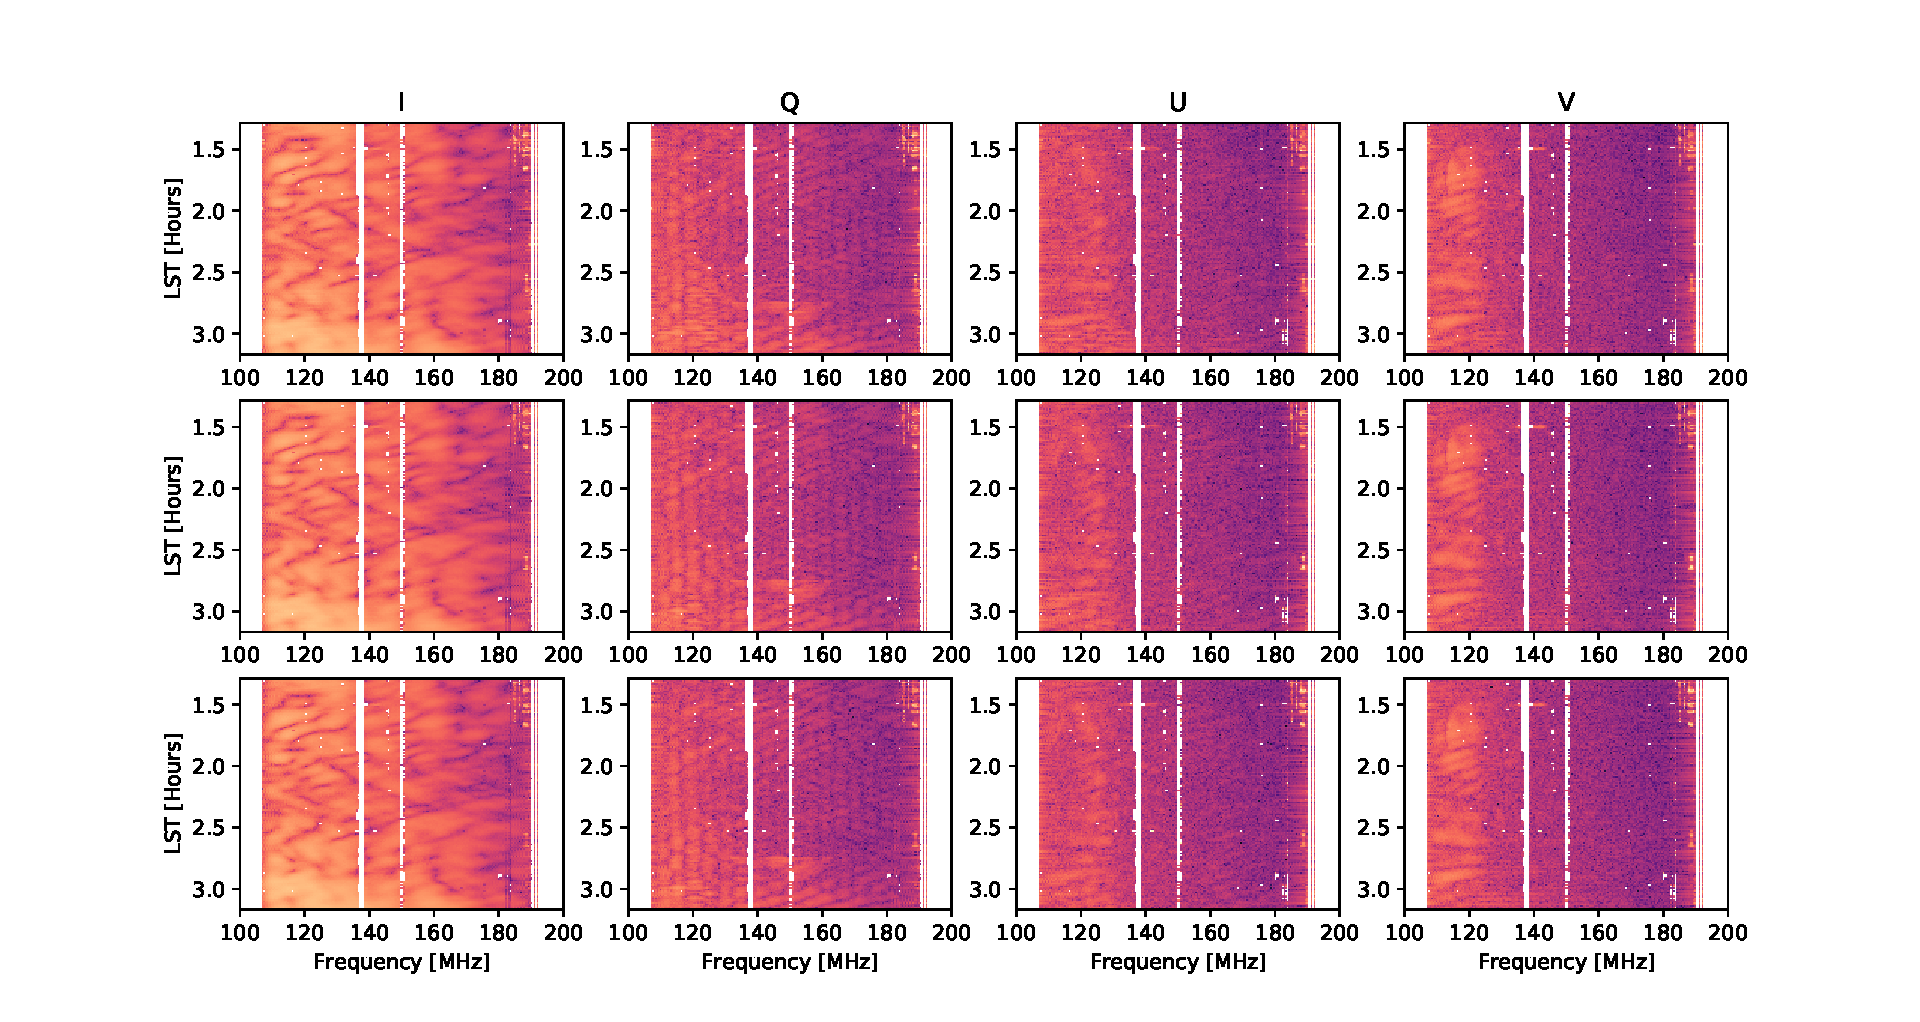
\includegraphics[width=0.8\textwidth]{chapters/psa128_pol/figures/omnical_IQUV_6680_0-5.pdf}
\caption[Amplitudes of three redundant visibilities before and after {\sc omnical}ibration using the \textit{4pol+minV} scheme.]{Amplitudes of three redundant visibilities before (above) and after (below) {\sc omnical}ibration using the \textit{4pol+minV} scheme. All four pseudo-Stokes polarizations attained a high degree of redundancy in magnitude after calibration. The color axis is logarithmic and spans 5 orders of magnitude in arbitrary data units.}
\label{fig:psa128_pre_post_abs}
\end{figure}

\begin{figure}
\centering
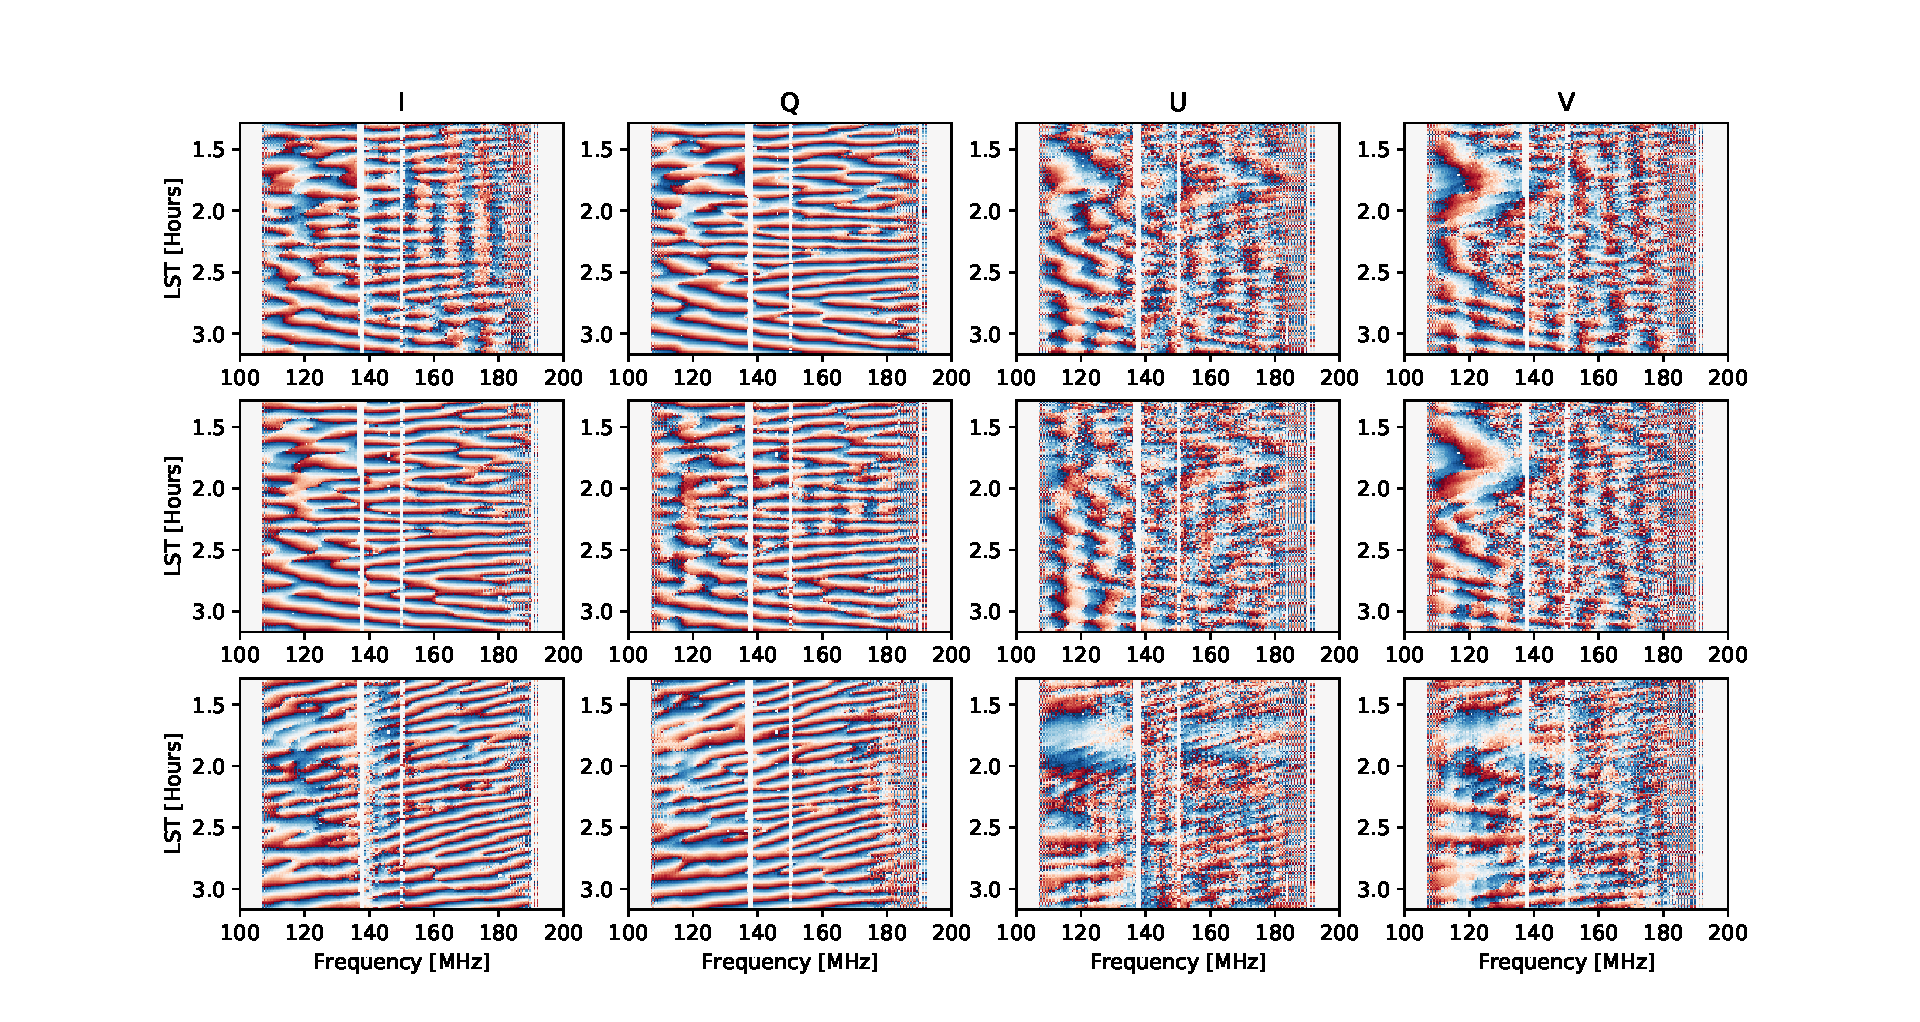
\includegraphics[width=0.8\textwidth]{chapters/psa128_pol/figures/nocal_IQUV_6680_phase.pdf}
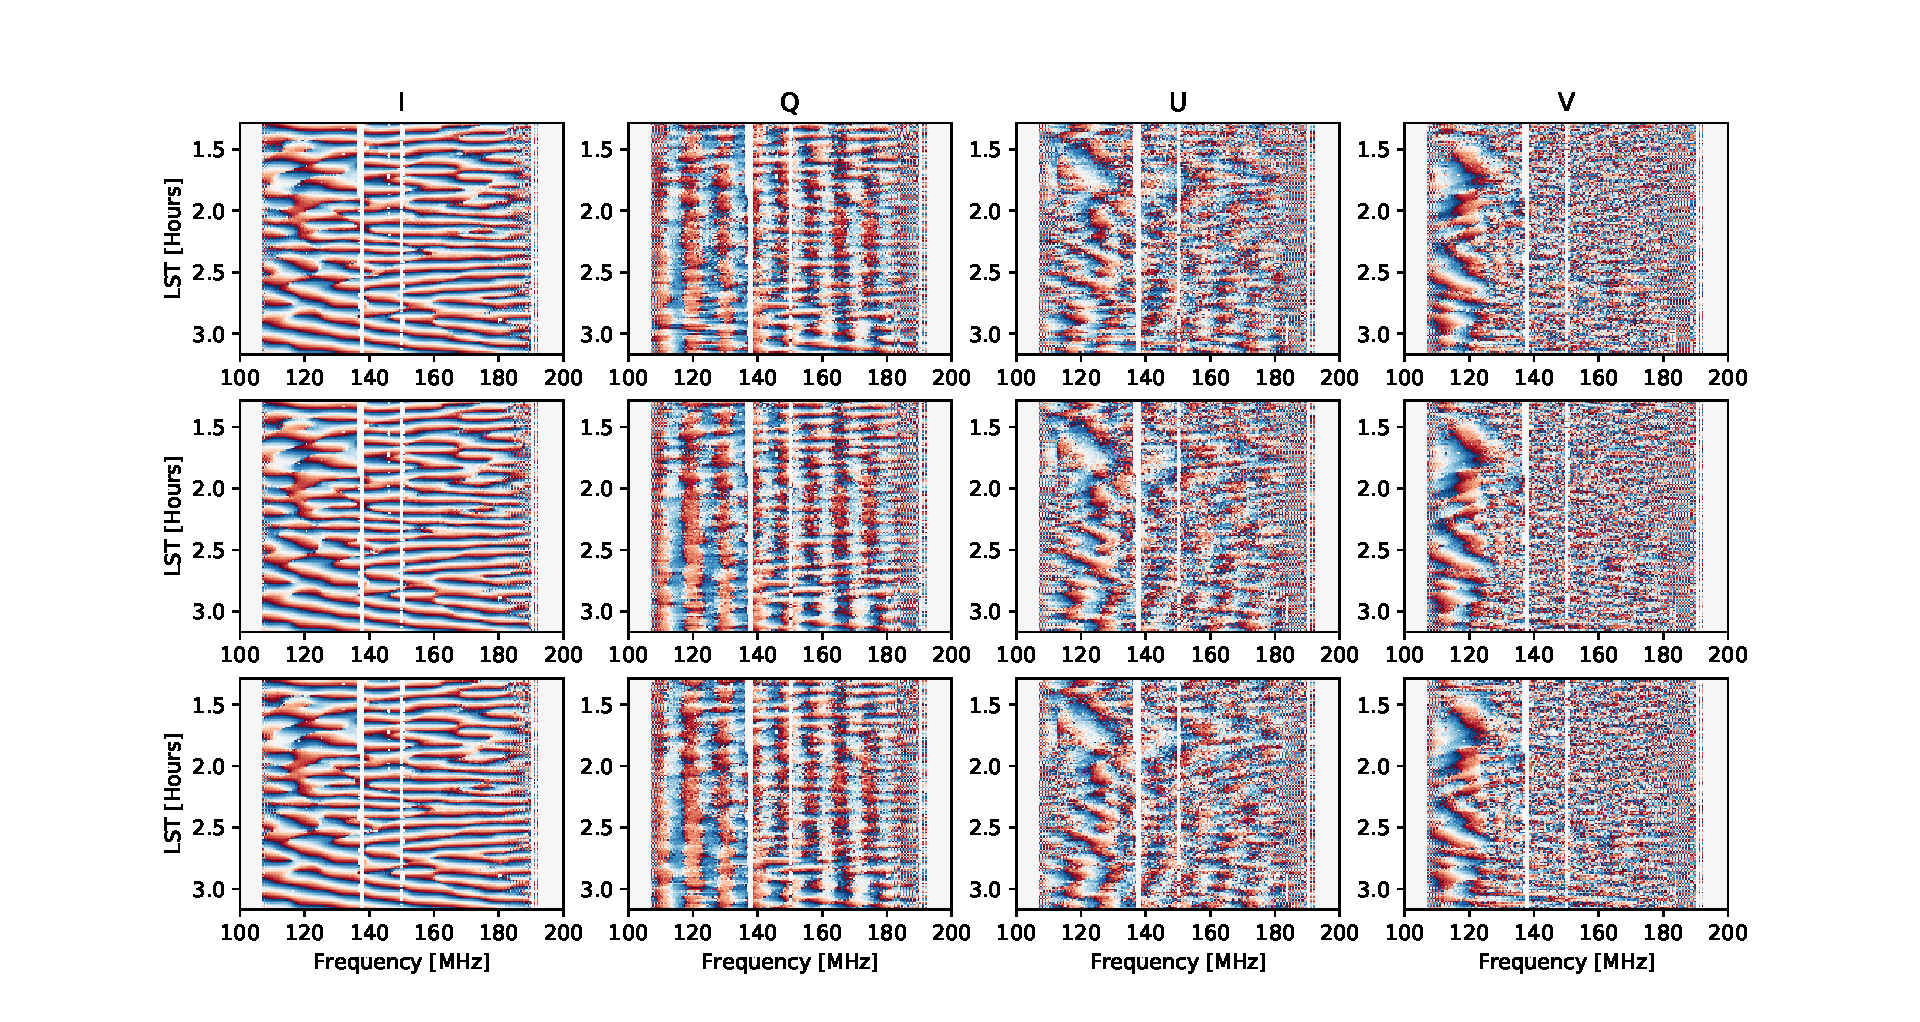
\includegraphics[width=0.8\textwidth]{chapters/psa128_pol/figures/omnical_IQUV_6680_phase.pdf}
\caption[The same visibilities as shown in Figure~\ref{fig:psa128_pre_post_abs}, but showing their phases instead of their amplitudes.]{The same visibilities as shown in Figure~\ref{fig:psa128_pre_post_abs}, but showing their phases instead of their amplitudes. Again, a high degree of redundancy is obtained between baselines for all polarizations. The color axis is linear and spans $\pi$ (red) to $-\pi$ (blue) radians.}
\label{fig:psa128_pre_post_phs}
\end{figure}

After calibration, we down-selected to only the baselines we sought to analyze for our power spectrum studies. This was partly a utilitarian step: reducing the entire data set would represent a large feat of data processing, since Season 1 Epoch 2 was $\sim2.5$ TB in size if all baselines were retained, and several processing stages that would duplicate the data were still required. The baselines kept were the 30\,m East-West type and their closest diagonals -- that is, 30\,m East-West \& $\pm$4\,m North-South baselines ({\color{red} e.g. Kolopanis et al. (2018)}).

\subsubsection{Foreground removal}
% - linCLEAN
To remove foreground signal from the data, we implemented a variation of the 1D-CLEAN \citep{ParsonsBacker.09} used by past PAPER studies \citep[][{\color{red}; Kolopanis et al. 2018}]{Parsons.14, Ali.15, Jacobs.15, Moore.17, Kerrigan.18}. Instead of performing an iterative CLEAN we used a linear least-squares approach which we termed {\tt linCLEAN}.

Using {\tt linCLEAN}, we endeavoured to model the foreground component of the visibilities using the finite number of Fourier modes that exist within the foreground wedge of the EoR window paradigm. The number of these modes was set by the frequency resolution of the instrument, and the baseline length (see Chapter~\ref{chapter:eor_window_theory}).
The Fourier conjugate of the frequency axis, known as the delay axis, is specified through the delay transform of a visibility, which for short baselines may be written as \citep{Parsons.12b}:

\begin{equation}
\tilde{V}(\tau) = \int^{\nu_{\rm max}}_{\nu_{\rm min}} V(\nu) \exp\left(2\pi i \tau \nu\right) {\rm d}\nu
\end{equation}
for visibility $V(\nu)$ and delay mode $\tau$. Delay modes become estimators for the Fourier-transformed brightness temperature field.

We constructed a visibility $\vec{m}(\nu)$ as a model, per time integration, of an individual visibility $\vec{d}(\nu)$ (which we represent as a vector along the frequency axis), seeking to minimize the chi-square

\begin{equation}
\chi^2(\nu) = (\vec{d}(\nu) - \textbf{A}(\nu',\tau)\vec{m}(\nu))^T \textbf{W}(\nu',\nu)(\vec{d}(\nu) - \textbf{A}(\nu,\tau)\vec{m}(\nu)).
\label{eq:linclean_chisquare}
\end{equation}

In the above equation, the matrix $\textbf{A}$ had dimensions ``number of frequency channels" by ``number of allowed delay modes". An allowed delay mode $\tau$ was within the interval [0,  $\frac{|\vec{b}|}{c} + t_{SH}$], for baseline vector $\vec{b}$, speed of light $c$ and an allowed ``supra-horizon leakage" term $t_{SH}$ \citep{Pober.13}, which we set to 15ns.

The contents of $\textbf{A}$ were the concatenation of matrices $\textbf{C}$ and  $\textbf{S}$:
\begin{eqnarray}
\textbf{C}_{ij} &=  \cos(2\pi \nu_i \tau_j)\\
\textbf{S}_{ij} &=  \sin(2\pi \nu_i \tau_j)\\
\end{eqnarray}
for frequency channel $i$ and delay bin $j$.
The matrix $\textbf{W}$ was diagonal, and assigned weighting per frequency channel. With an estimated system temperature one could implement an inverse variance weighting per frequency channel, but we pursued a simpler scheme where the entries were zero for RFI-flagged channels, and unity otherwise.

This system was least-squares solvable for the delay modes, and granted a foreground model

\begin{equation}
\vec{m}(\nu) = (\textbf{A}^T \textbf{W} \textbf{A})^{-1}\textbf{A}^T\textbf{W}\vec{d}(\nu)
\end{equation}
which could subsequently be subtracted from the $\vec{d}(\nu)$, leaving only the noise-like backgrounds.

We ran {\tt linCLEAN} on the Epoch of {\sc omnical}ibrated data, using the entire unflagged part of the band (for details on flagging of PAPER-128 data, see Chapter~\ref{chapter:data_prep_and_proc}) to obtain an estimate of $\textbf{A}$.
After this, we implemented a round of RFI flagging that clipped any samples that represented $>4\sigma$ fluctuations above the average, where averages were performed along the time and frequency axes.

\subsubsection{Binning in LST}

We could then average-down on the noise by binning visibilities according to the LST they were observed at. The LST bin size used was 41s long, and we split the Epoch into even and odd days, constructing two separate LST-binned data sets. Cross-multiplying these allowed us to construct an unbiased power spectrum estimate \citep[e.g.][{\color{red}; Cheng et al. 2018}]{Parsons.14}.
Unflagged RFI events would dominate any other signal in a given LST bin. To avoid binning RFI with sky signal, before averaging we computed the median of all observations in a given LST bin and flagged any observations with amplitude $>3\sigma$ above the median. This clipping narrowed the distribution of visibilities about the median, altering the thermal noise variance, but leaving the expectation value unchanged, so we expect little loss of signal due to this step.

For this analysis, we created two LST-binned data sets (each split into even and odd days): a set constructed from the foreground subtracted visibilities, and another set with the foregrounds included. We used the latter to calculate an absolute calibration of both data sets.

\subsubsection{Absolute calibration \& fringe-rate filtering}
% - (unpolarized) PicA (Jacobs13) CASA cal on lstbin_fg
% - Stokes I FRF on all 4pols of fgsub
We formed images of the Pictor A transit in order to derive an absolute calibration for the `n' and `e' feed arms in the fashion described in Chapter~\ref{chapter:polcal}. We converted the {\sc miriad} files of the LST-binned foreground data into {\tt CASA} \citep{casa} Measurement Sets at LST$\approx$5.3 hours (the relevant LST for the transit of Pictor A). 
Our sky model consisted only of Pictor A as a unpolarized point source. Because we had already down-selected to the power spectrum baselines, Pictor A completely dominated the signal. The images of the four pseudo-Stokes parameters we obtained are shown in Figure~\ref{fig:psa128_abscal_images}. In that image, pseudo-Stokes I is on a color scale with double the dynamic range of Q, U and V -- that is, pseudo-Stokes Q, U and V were almost completely noise-like. In pseudo-Stokes I, Pictor A dominated the field. These images were low quality because only the power spectrum baselines were used to produce the image, leading to large grating lobes and an elongated point-spread function; shown in Figure~\ref{fig:psa128_psf}.

\begin{figure}
\hspace{-2cm}\begin{tabular}{ll}
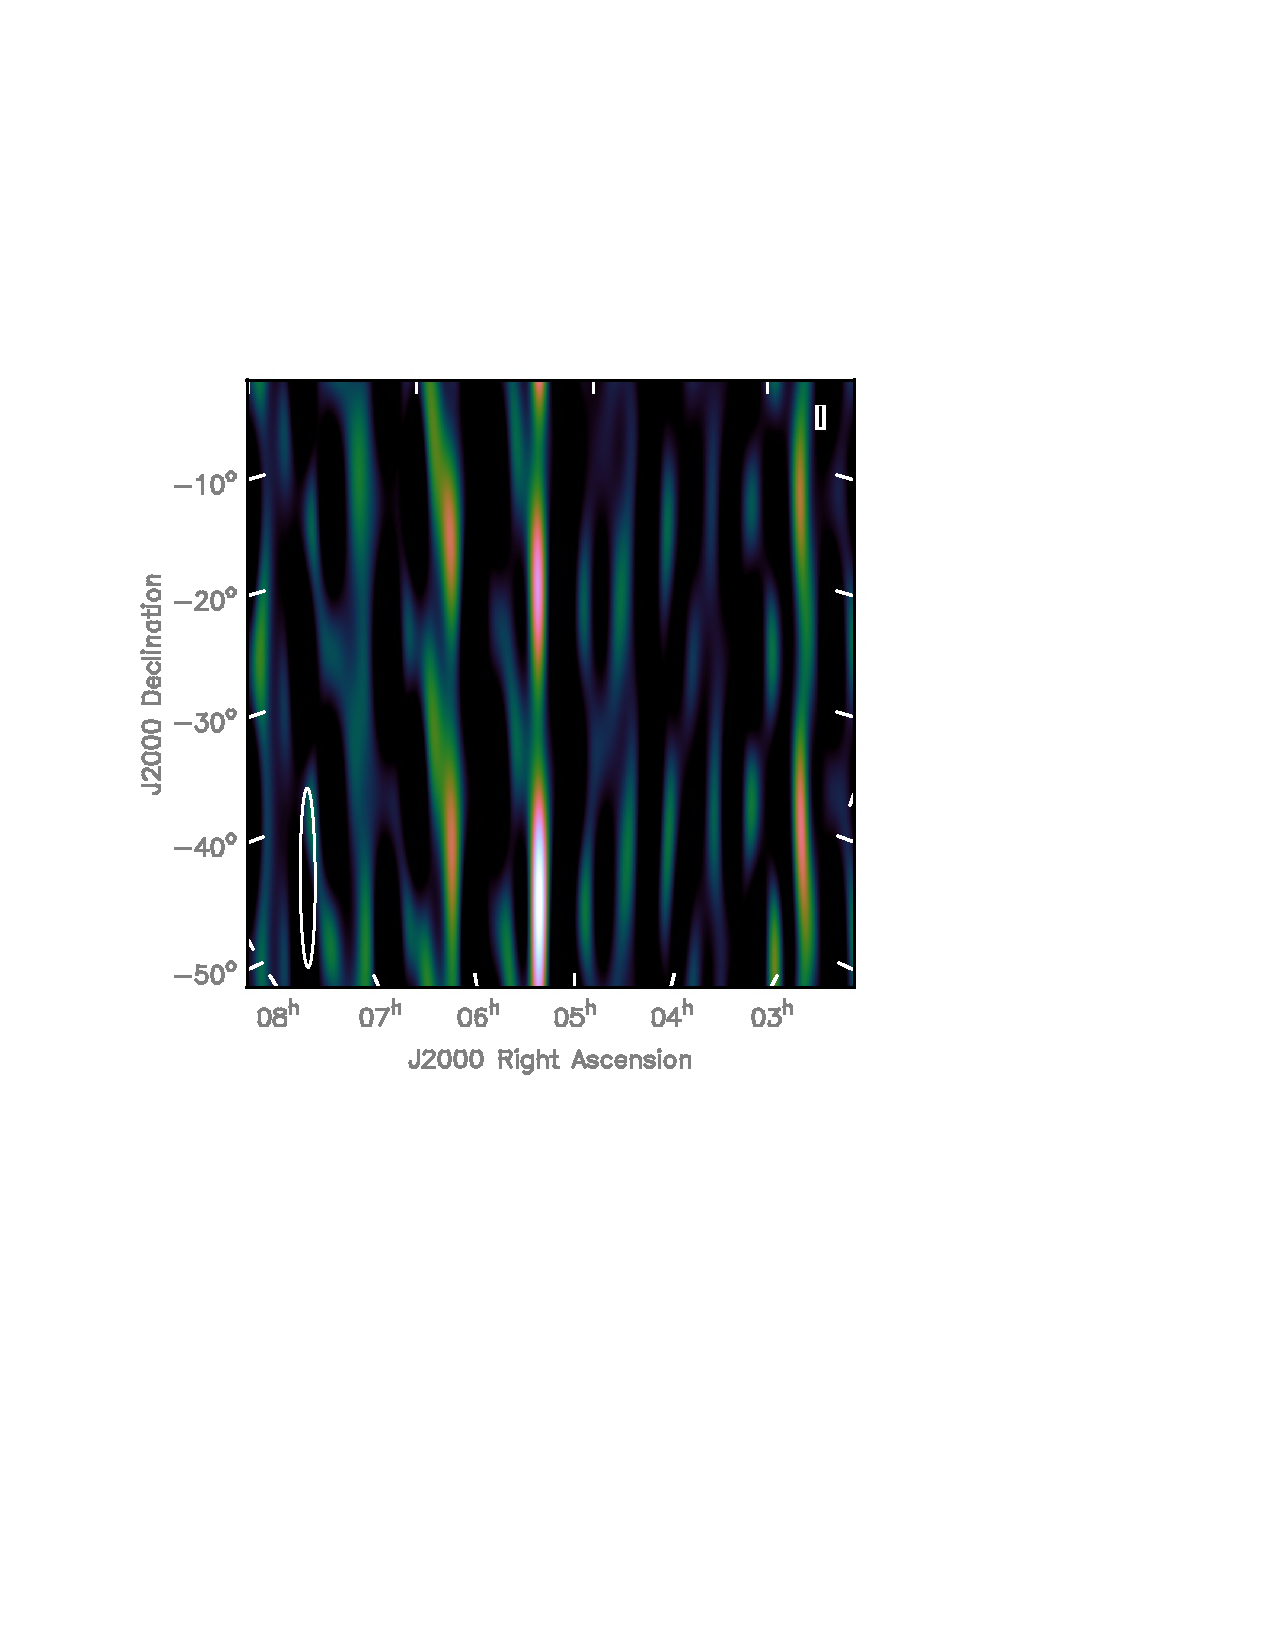
\includegraphics[clip, trim=0.5cm 9cm 5cm 5cm, width=0.6\textwidth]{chapters/psa128_pol/figures/pretty_I_0-022.pdf} &
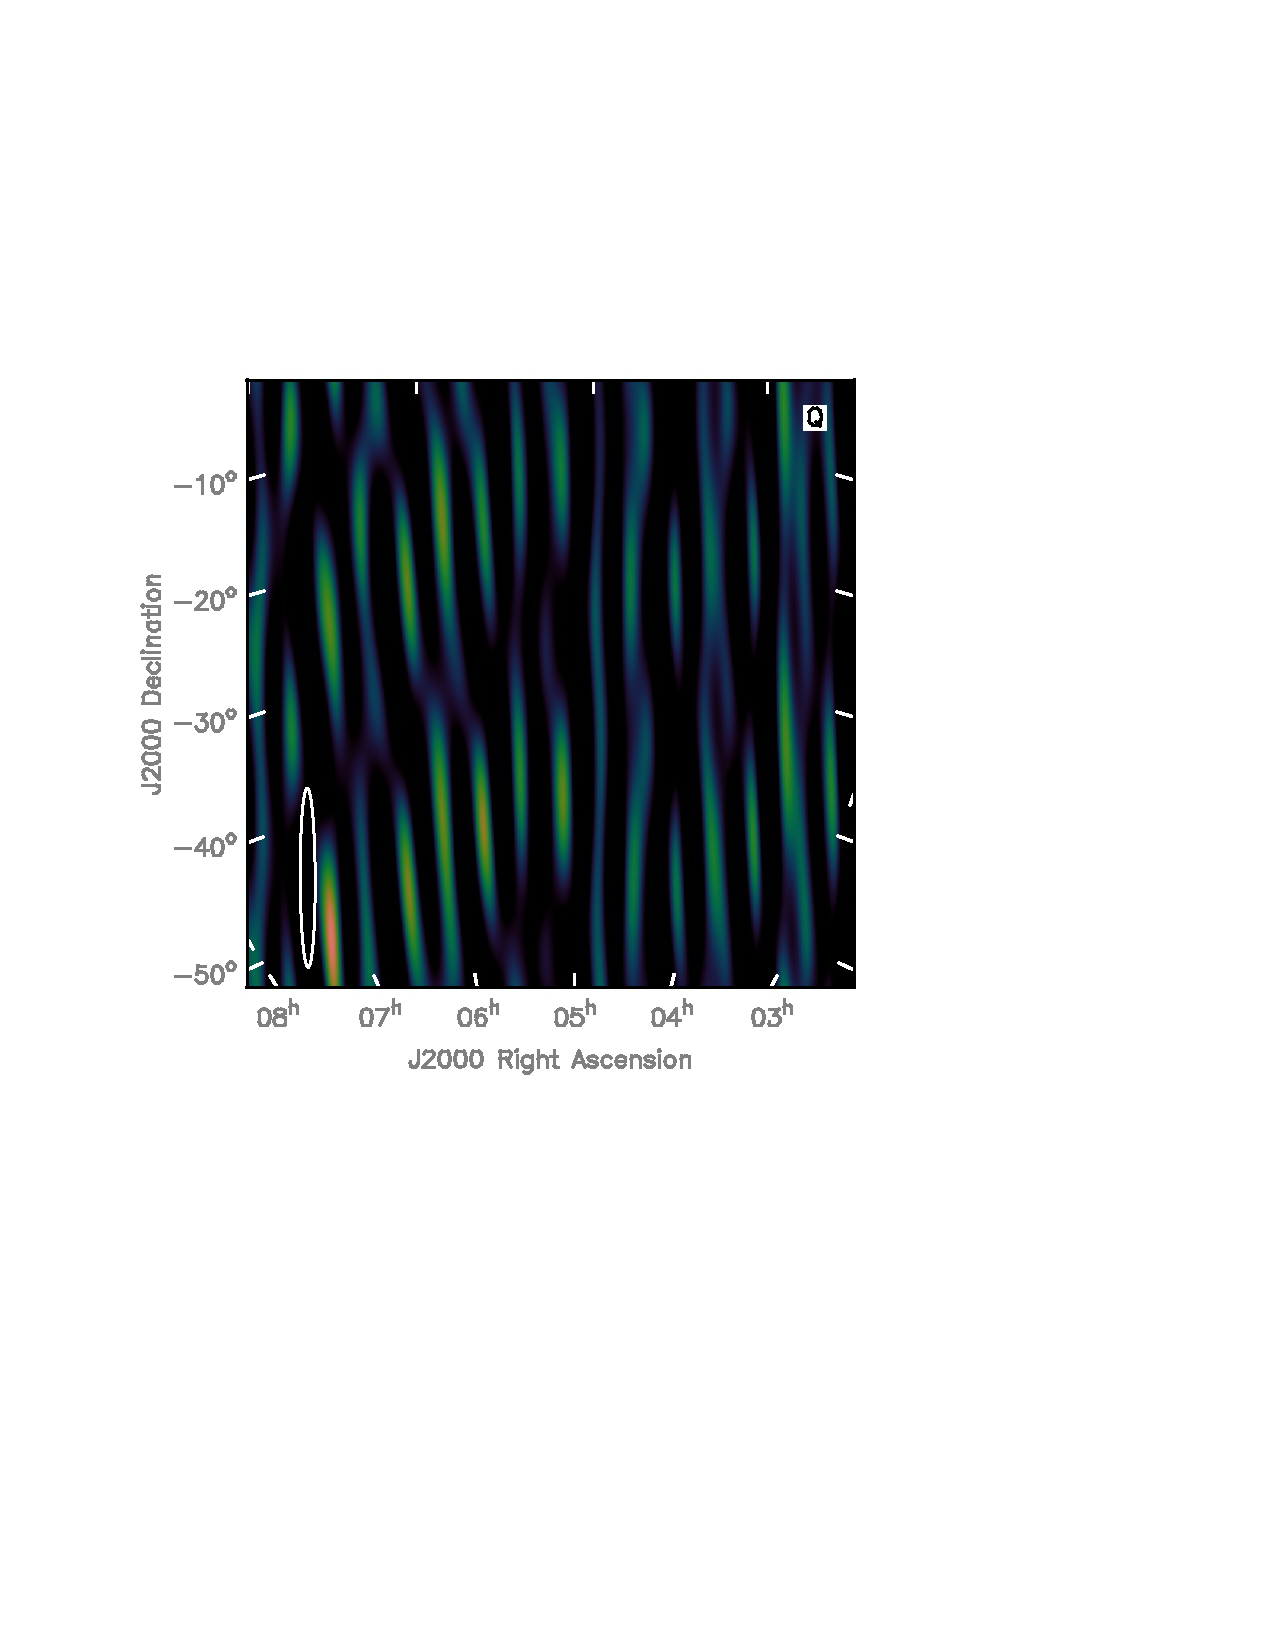
\includegraphics[clip, trim=0.5cm 9cm 5cm 5cm, width=0.6\textwidth]{chapters/psa128_pol/figures/pretty_Q_0-011.pdf}\\
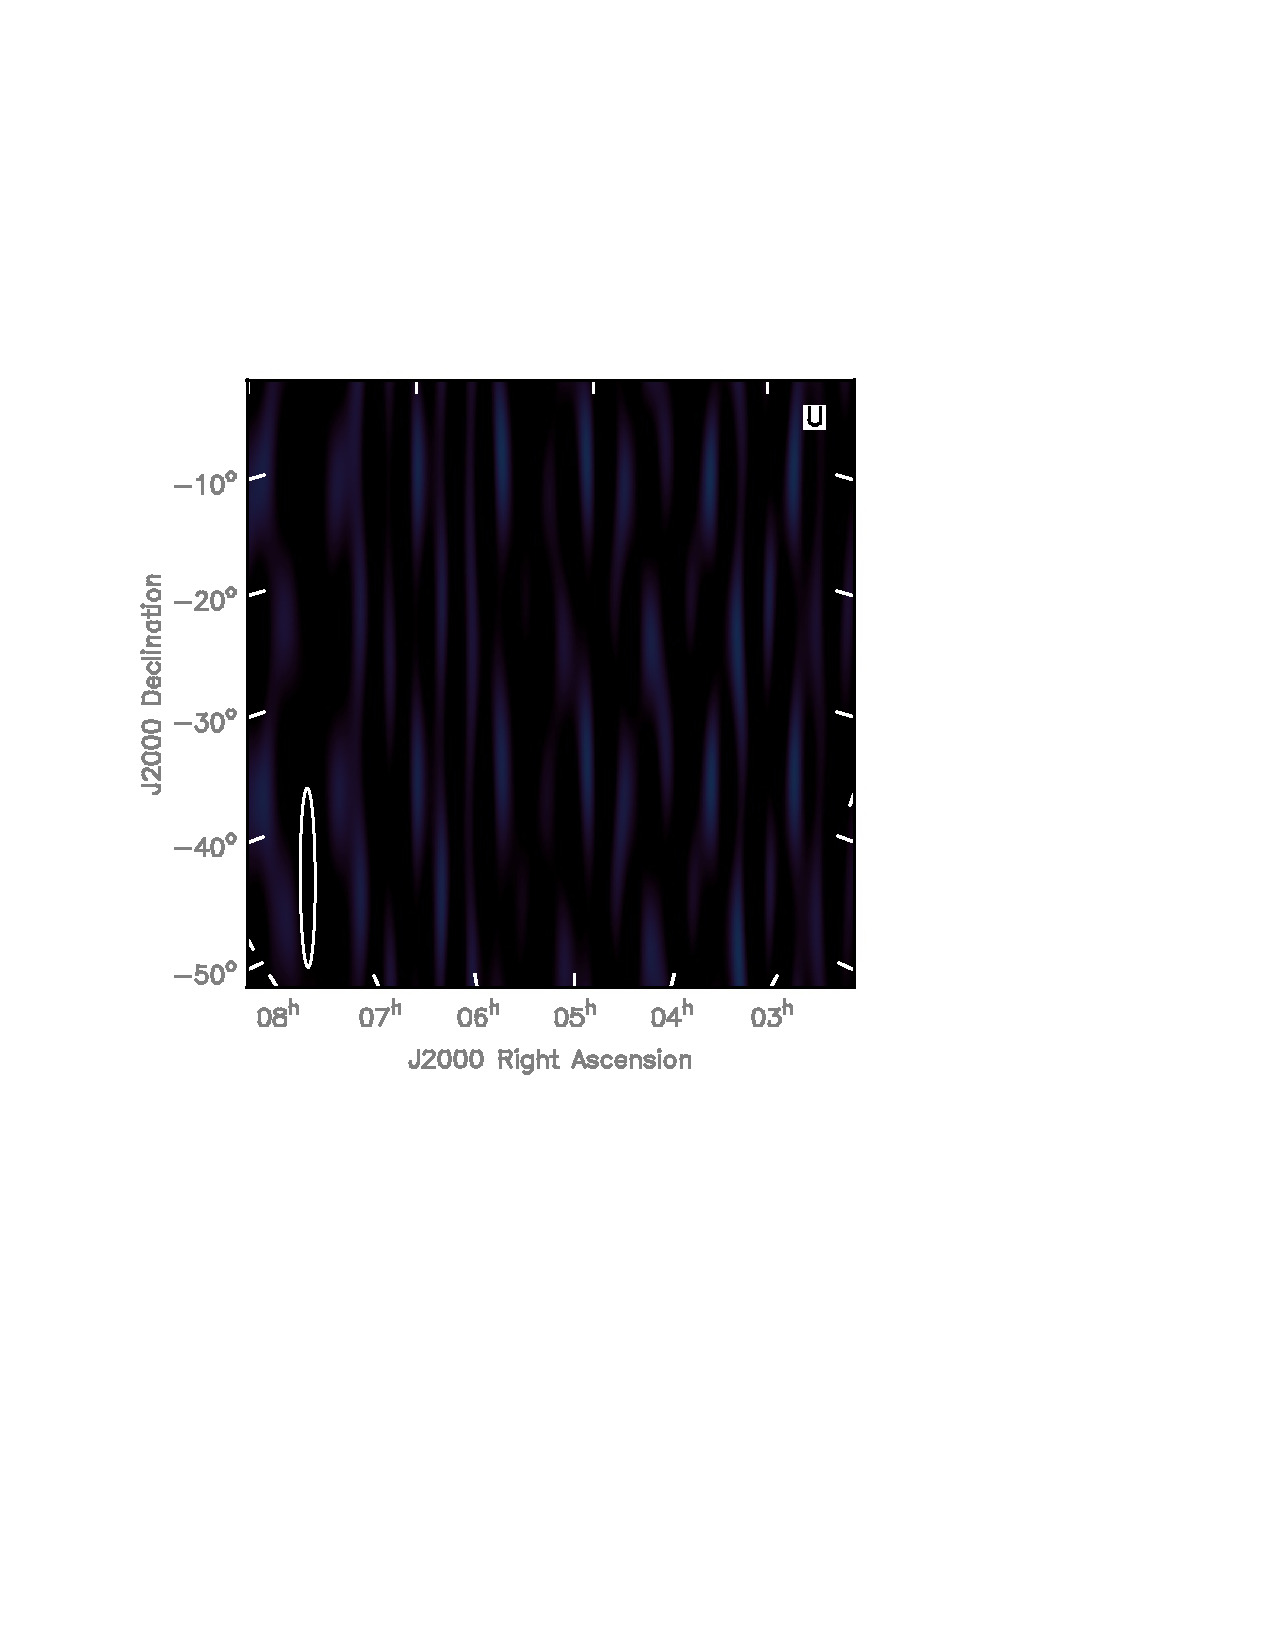
\includegraphics[clip, trim=0.5cm 9cm 5cm 5cm, width=0.6\textwidth]{chapters/psa128_pol/figures/pretty_U_0-011.pdf} &
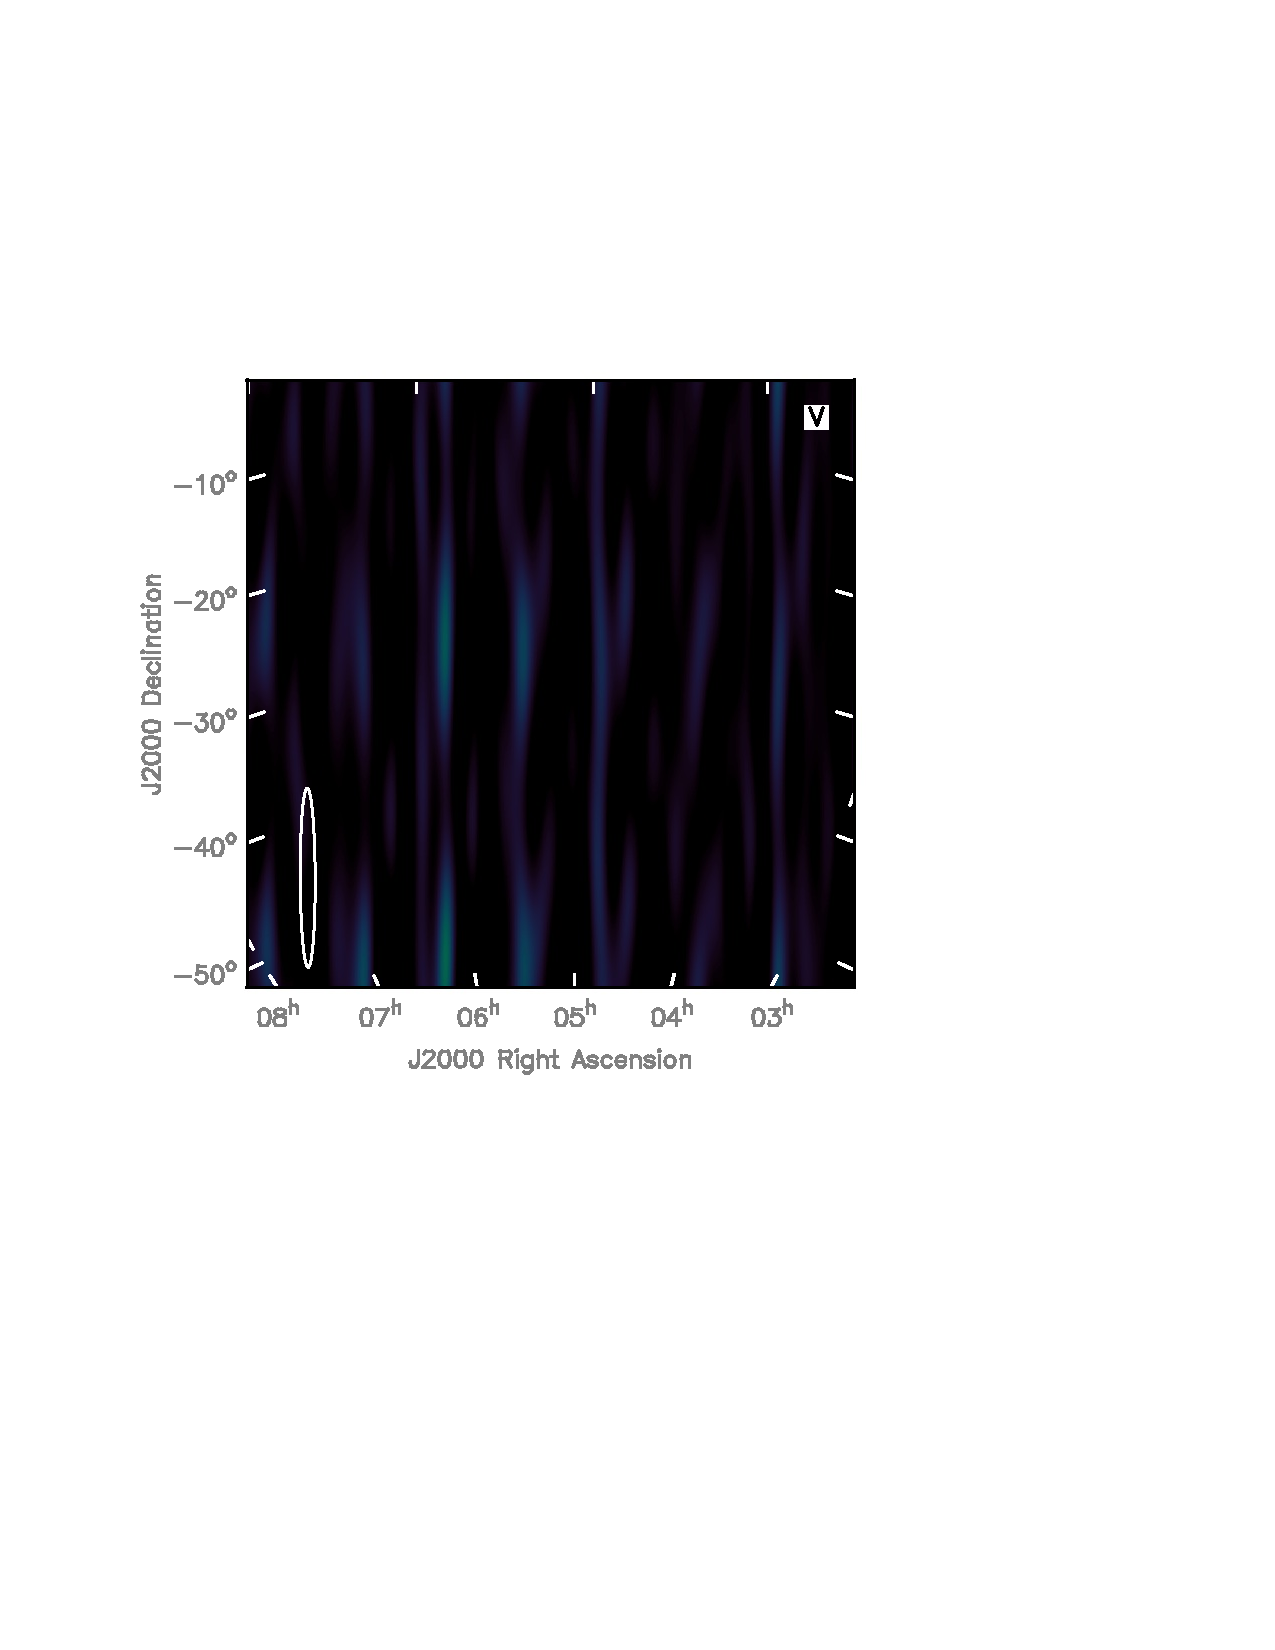
\includegraphics[clip, trim=0.5cm 9cm 5cm 5cm, width=0.6\textwidth]{chapters/psa128_pol/figures/pretty_V_0-011.pdf} \\
\end{tabular}
\caption[Images of Pictor A, used to calibrate the absolute scaling to physical units.]{Images of Pictor A, used to calibrate the absolute scaling to physical units. These images are multi-frequency syntheses, but we used per-channel information for the final calibration (see Figure~\ref{fig:psa128_bandpases}). 
Pseudo-Stokes I is on a linear scale of twice the dynamic range of pseudo-Stokes Q, U and V. A beam ellipse is shown in the South-West corner of the images.
The poor quality of the images is a result of using only the baselines that go into the power spectrum estimates. Pictor A dominates the field in pseudo-Stokes I, and is of the morphology expected given the PSF shown in Figure~\ref{fig:psa128_psf}.}
\label{fig:psa128_abscal_images}
\end{figure}

\begin{figure}
\centering
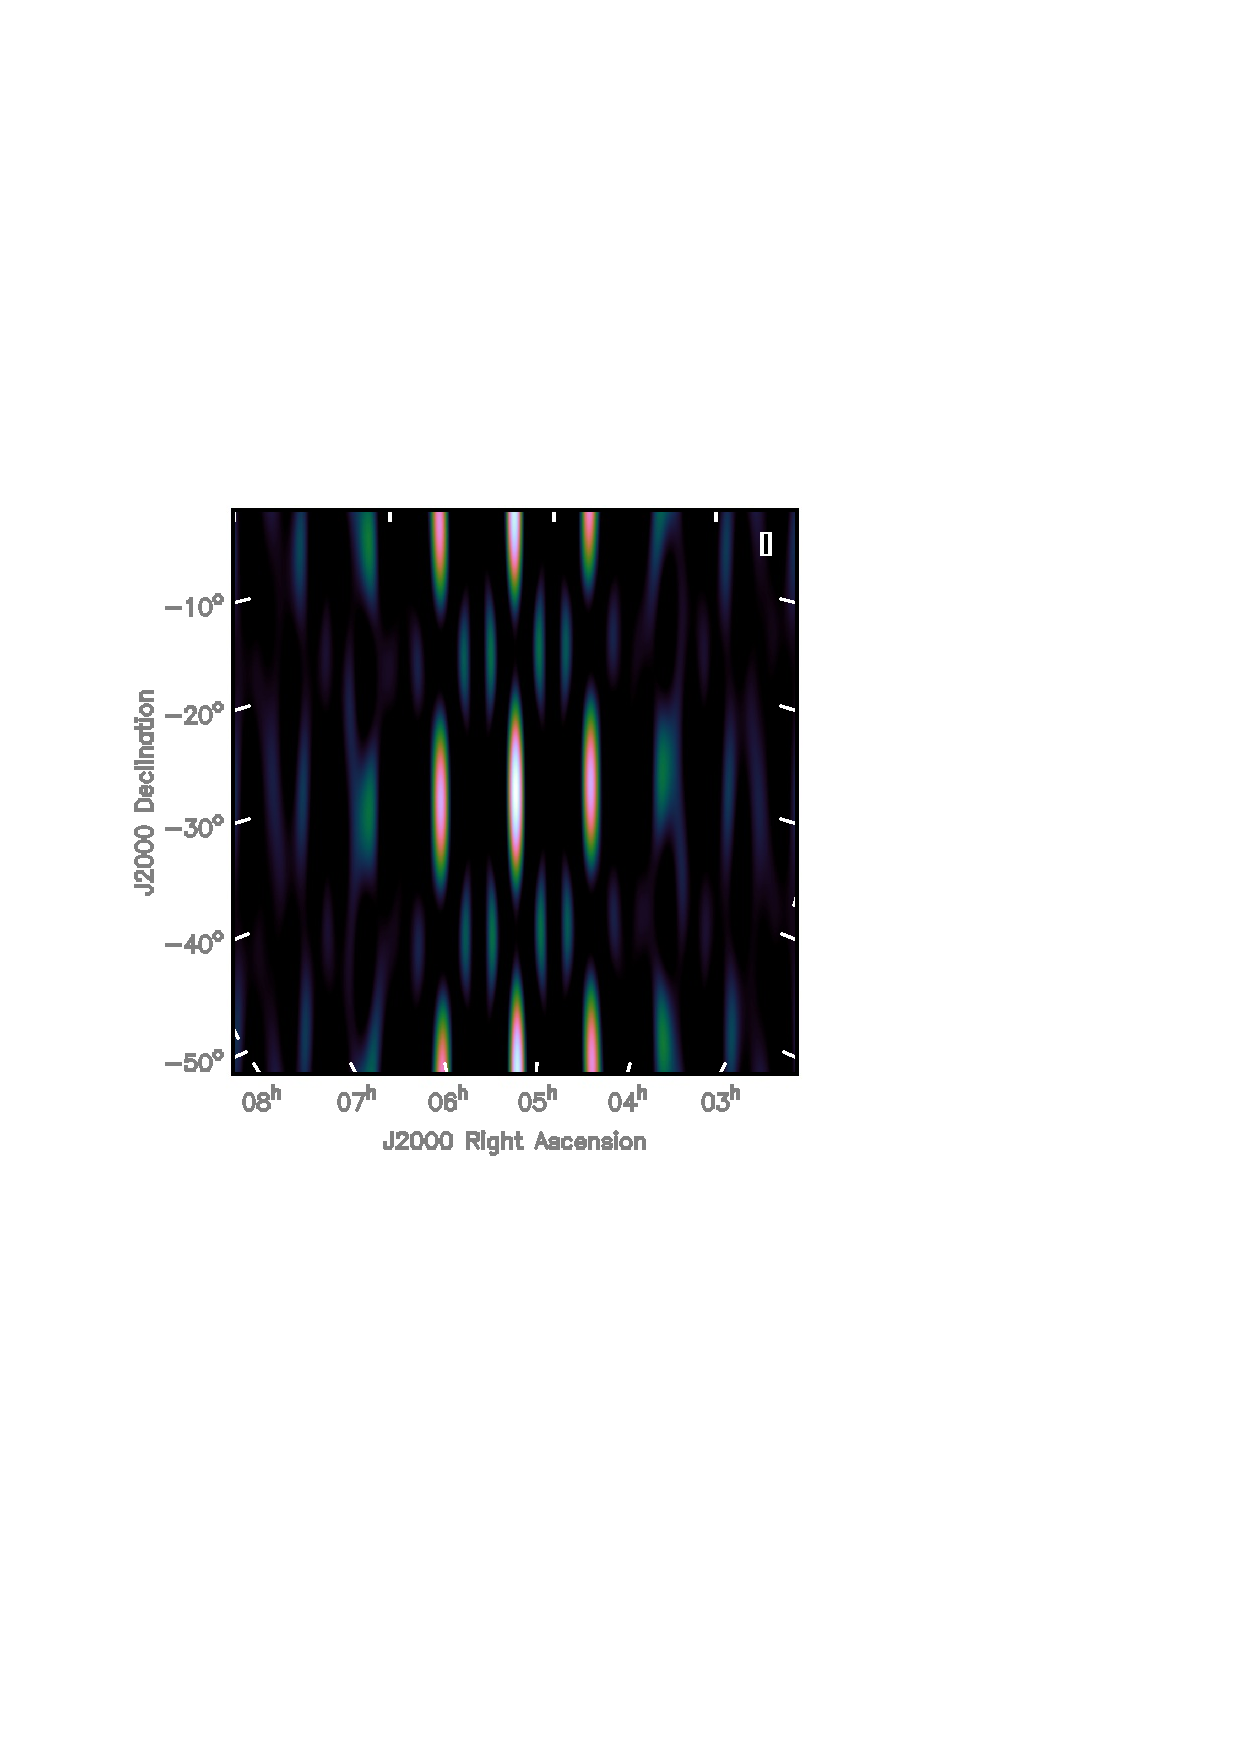
\includegraphics[clip, trim=0.5cm 9cm 5cm 5cm, width=0.6\textwidth]{chapters/psa128_pol/figures/pretty_PSF_0-1.pdf}
\caption[The point-spread function of an array consisting only of the $\sim$30\,m power spectrum baselines.]{The point-spread function of an array consisting only of the $\sim$30\,m power spectrum baselines. The sparseness and asymmetry of the array lead to an elongated PSF with large grating lobes.}
\label{fig:psa128_psf}
\end{figure}

We used the {\tt CASA} {\tt bandpass} routine to derive an overall frequency-dependent scaling that brought the North-South and East-West dipole arms to a physical scale that minimized pseudo-Stokes Q in Pictor A, and converted the data units to a physical level in Janskies. For the Jansky scaling we used the spectrum from \cite{Jacobs.13}. {\tt CASA} provided separate scalings for all antennas used in the analysis. We plot the average scaling for the North-South and East-West dipole arms in Figure~\ref{fig:psa128_bandpases}, shading-in the standard deviation between antennas. We implemented aggressive RFI flags, leading to large gaps in the spectrum. The higher frequency portion of the band had a very low variance its bandpass solutions, as expected given that they were {\sc omnical}ibrated and that the low band was historically poorly-behaved and characterized (e.g. Chapter~\ref{chapter:polcal}).

\begin{figure}
\centering
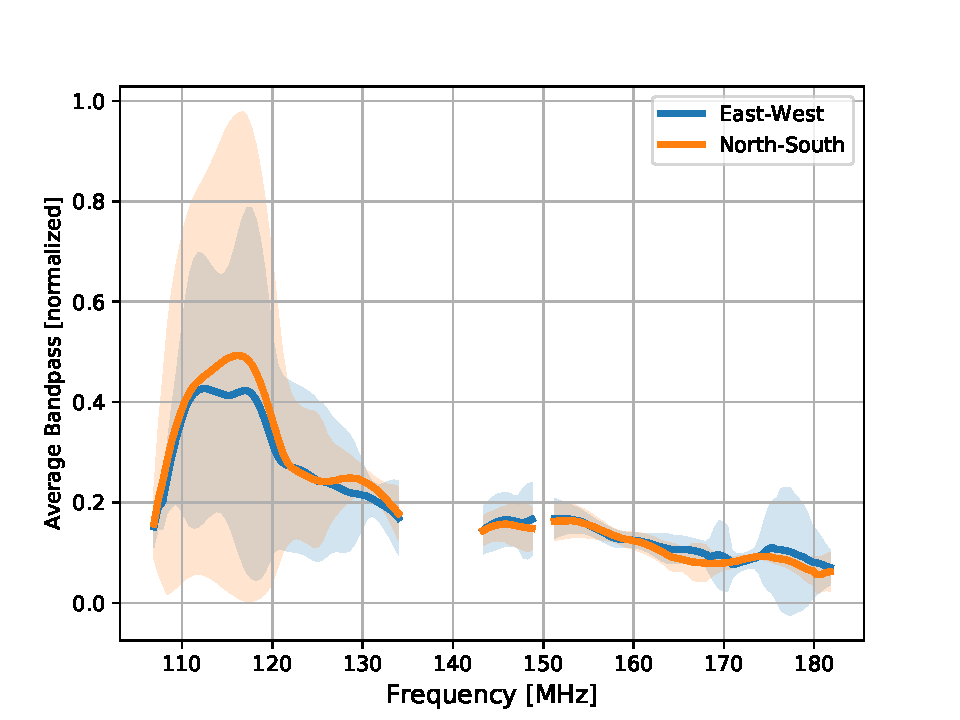
\includegraphics[width=0.8\textwidth]{chapters/psa128_pol/figures/avg_bandpasses.pdf}
\caption[The average bandpass scaling used for absolute calibration.]{The average bandpass scaling used for absolute calibration, with shading indicating the 1$\sigma$ deviation about the average across antennas.}
\label{fig:psa128_bandpases}
\end{figure}

As discussed in Chapter~\ref{chapter:data_prep_and_proc}, every baseline not only samples characteristic delay modes based on its length, but also characteristic modes in time, per frequency, known as `fringe rates' \citep[if frequency dependence is ignored, they are referred to as ``delay rates"; e.g.][]{ParsonsBacker.09}. For drift-scan telescopes such as PAPER, the sky, beam and fringe terms are locked to one another and can be thought of as an enveloped fringe pattern which varies in time as the Earth rotates. The rate of of change of this pattern -- the fringe rate -- depends only on the baseline length (which gives the fringe width) and the position of the drift-scanning telescope on Earth. By Fourier-transforming along the time axis of recorded visibilities, one can identify a ``window" of physical Fourier modes that represent fringe rates reflective of the Earth's rotation. Such a window is shown for a 30\,m single baseline in Figure~\ref{fig:fringerate_example}. By convolving an appropriate filter, one could extract these physical fring rates and filter-out noise. This is equivalent to changing the shape of the primary beam of an antenna after observation, and was explored in \cite{Parsons.15}, and implemented in \cite{Ali.15}. However, because the range of physical fringe rates for a short baseline is narrow, this amounts to correlating a large number of visibility measurements in time, which must be accounted for in signal-to-noise estimates \citep[][{\color{red} Cheng et al. (2018)}]{Ali.15}.

\begin{figure}
\centering
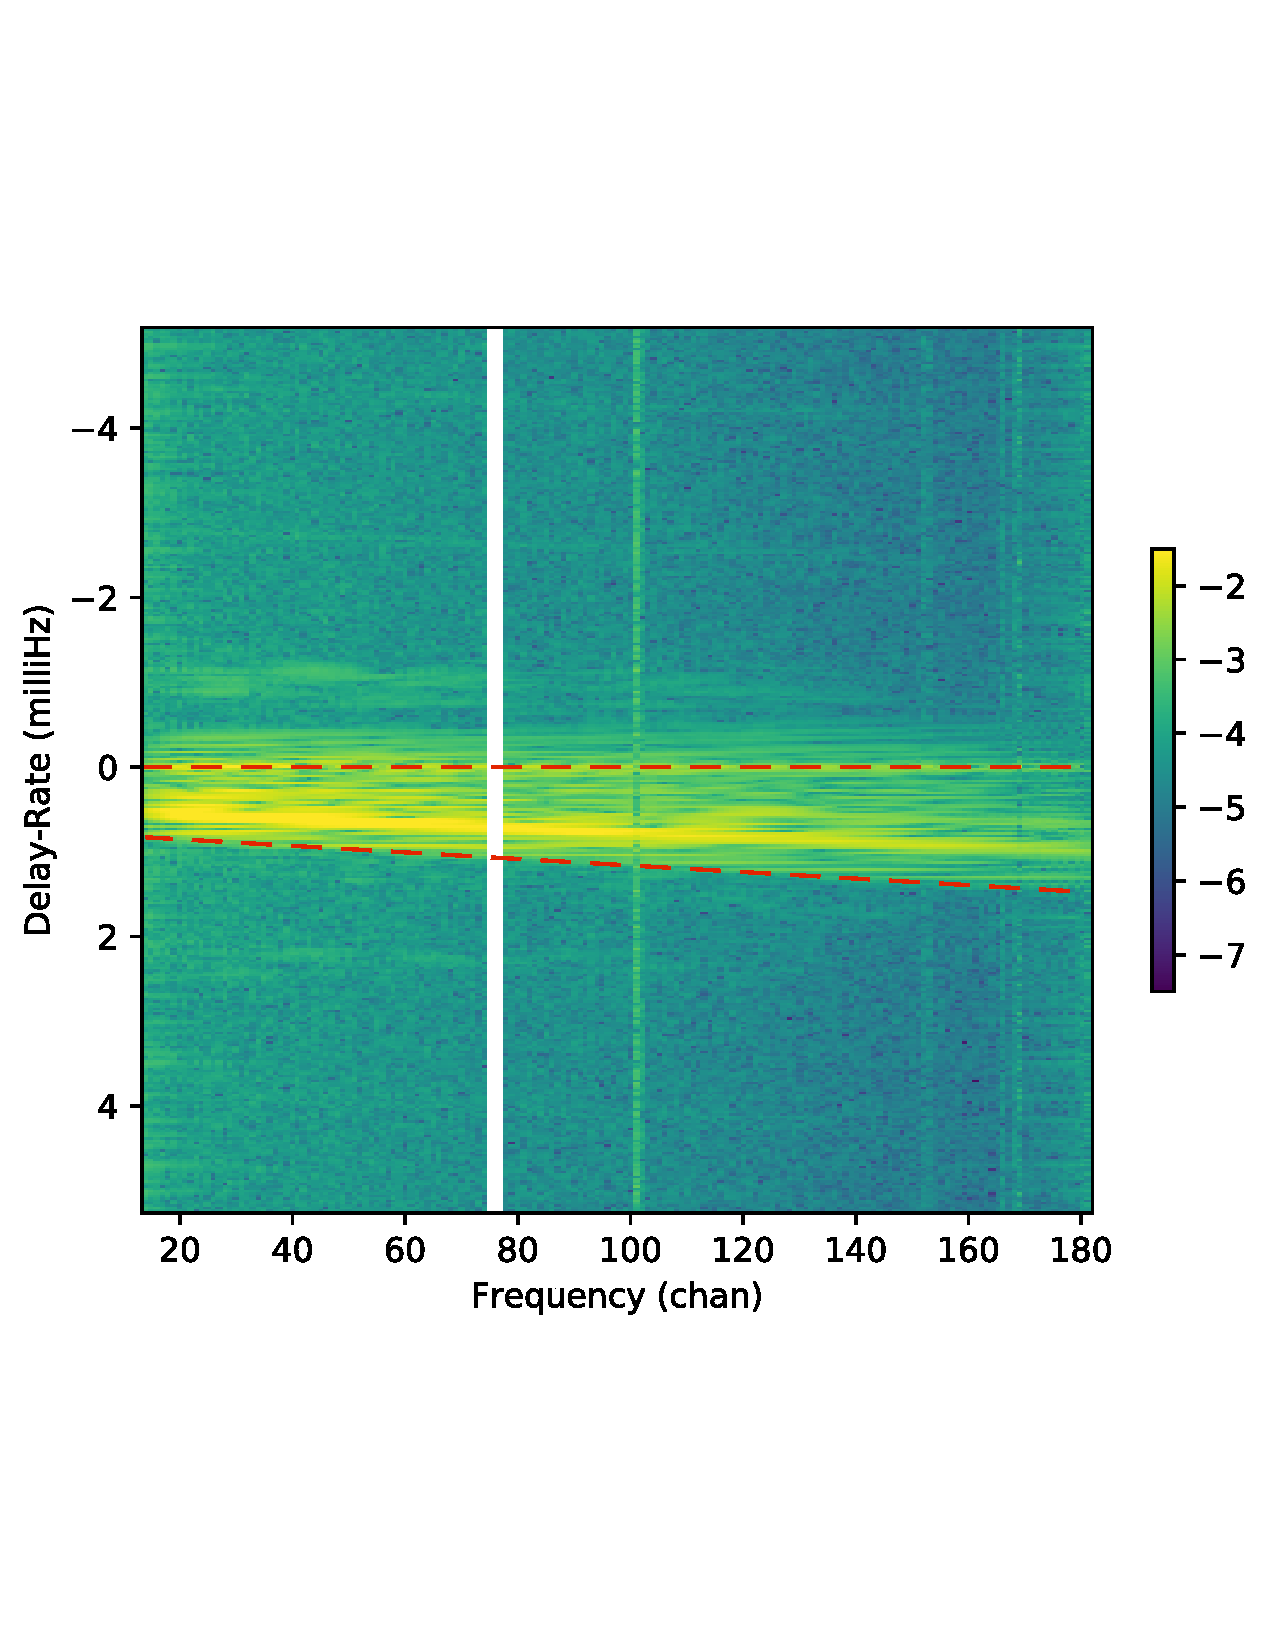
\includegraphics[width=0.5\textwidth]{chapters/psa128_pol/figures/fringerate_example.pdf}
\caption[Delay-rate vs. frequency for a 30\,m baseline in the `xx' (East-East) polarization.]{Delay-rate vs. frequency for a 30\,m baseline in the `xx' (East-East) polarization. The color axis is logarithmic, in arbitrary data units -- there is a clear ``window" of delay-rate modes of high amplitude. These correspond to physical modes to do with the Earth's rotation. The rest of the delay-rates are simply noise-modes and can be filtered-out.}
\label{fig:fringerate_example}
\end{figure}

We implemented such a filter on the LST-binned and absolute-calibrated background data, and proceeded to form power spectra.

\subsection{Forming power spectra}

As shown in Figures~\ref{fig:psa128_pre_post_abs} and \ref{fig:psa128_bandpases}, the 150--180 MHz section of the band had lower noise and a more precise calibration. Within this, we down-selected to the 10\,MHz-wide 155--165 MHz sub-band to form power spectra. This bandwidth was appropriate for an EoR analysis, since the {\sc hi} signal is to a reasonable approximation coeval over the corresponding redshift range \citep{Furlanetto.06}. The central redshift our frequencies corresponded to was $z=8.07$ (we assumed the \cite{Planck.16} cosmological parameters throughout this Chapter).

Power spectrum estimators per baseline and time were formed by cross-multiplying delay-transformed visibilities between even and odd days, at identical $\tau$ modes and LSTs:

\begin{equation}
\hat{P}_{ij}(\tau, t) = \left(\frac{\lambda^2}{2k_B}\right)^2 \frac{X^2Y}{\Omega_{PP}\Delta\nu} \left\langle \tilde{V}^{\rm* P, even}_{ij}(\tau,t) \tilde{V}^{\rm P, odd}_{ij}(\tau,t) \right\rangle.
\end{equation}
Above, $\hat{P}_{ij}(\tau, t)$ is an estimate of the power spectrum for baseline $ij$, for delay mode $\tau$ at LST $t$. The $\lambda^2/2k_B$ term is the conversion from Jansky to Kelvin, $\Omega_{PP}$ is the solid angle of the squared primary beam, $\Delta\nu$ is the 10\,MHz bandwidth and $X^2Y$ is the conversion from observed volume $\Omega_{PP}\Delta\nu$ to cosmological volume in $h^{-3}$Mpc$^3$ \citep{Parsons.12b}. $\tilde{V}^{\rm* P, even}_{ij}$ indicates the delay-transformed visibility for baseline $ij$, conjugated, for pseudo-Stokes polarization $P$ within the ``even days" LST-binned data set.

Delay modes could be converted to $k_{\parallel}$ line-of-sight modes measured in $h$/Mpc following
\begin{equation}
k_{\parallel} = \frac{2\pi \nu_{\rm 21cm} H(z)}{c(1+z)^2}\tau,
\end{equation}
where $\nu_{\rm 21cm}\approx1420.1$\,MHz, and $H(z)$ is the Hubble parameter at redshift $z$. The angular cosmological distance surveyed was proportional to the magnitude of the baseline length $b$, represented in Fourier space by $k_{\perp}$:
\begin{equation}
k_{\perp} = \frac{2\pi}{D(z)\lambda}b
\end{equation}
where $D(z)$ is the transverse comoving distance at redshift $z$. For the $\sim$30\,m baselines used in this study, $k_{\parallel}>>k_{\perp}$. 

The spherically-averaged power spectrum estimate $\hat{P}(k)$ could be formed by averaging over LSTs and redundant baselines, where $k^2 = k_{\parallel}^2 + k_{\perp}^2$. These estimates in turn were averaged over the three separation types described in Section~\ref{subsubsec:psa128_redcal}. Uncertainties were estimated by bootstrapping over groups of redundant baselines and LST samples. Obtaining the correct uncertainties when bootstrapping from the data used to form the estimate is not a trivial process, and we defer the reader to {\color{red} Cheng et al. (2018)} for full details of this important step. 

Past PAPER power spectrum results have used inverse covariance-weighting and optimal quadratic estimators to improve the accuracy of the final power spectrum estimate \citep[e.g.][{\color{red}; Cheng et al. 2018}]{Parsons.14}. We do not implement any weighting in our power spectrum estimates. This avoided risk of signal-loss effects, but more generally avoided making any assumptions about the nature of the polarized sky. Down-weighting polarized foregrounds using optimal quadratic estimation is a contemporary analysis challenge that has not yet been implemented on data.

\section{Results}
\label{sec:psa128_results}

Figure~\ref{fig:psa128_power_spectra_data} shows the spherically-averaged power spectra for pseudo-Stokes I, Q, U and V with 95\% confidence intervals. Green curves show analytical thermal noise estimates drawn from a {\sc 21cmsense} model of the array \citep{Pober.14, cmsense} and given our observing time and bandwidth. The analytical thermal noise estimates used a simplistic model of the polarized beam, leading to different, but valid, noise levels per Stokes parameter. An equivalent series of power spectra based on Gaussian noise of the same variance as our data are shown in Figure~\ref{fig:psa128_power_spectra_noise}, as a consistency-check on our method.

\begin{figure}
\begin{tabular}{ll}
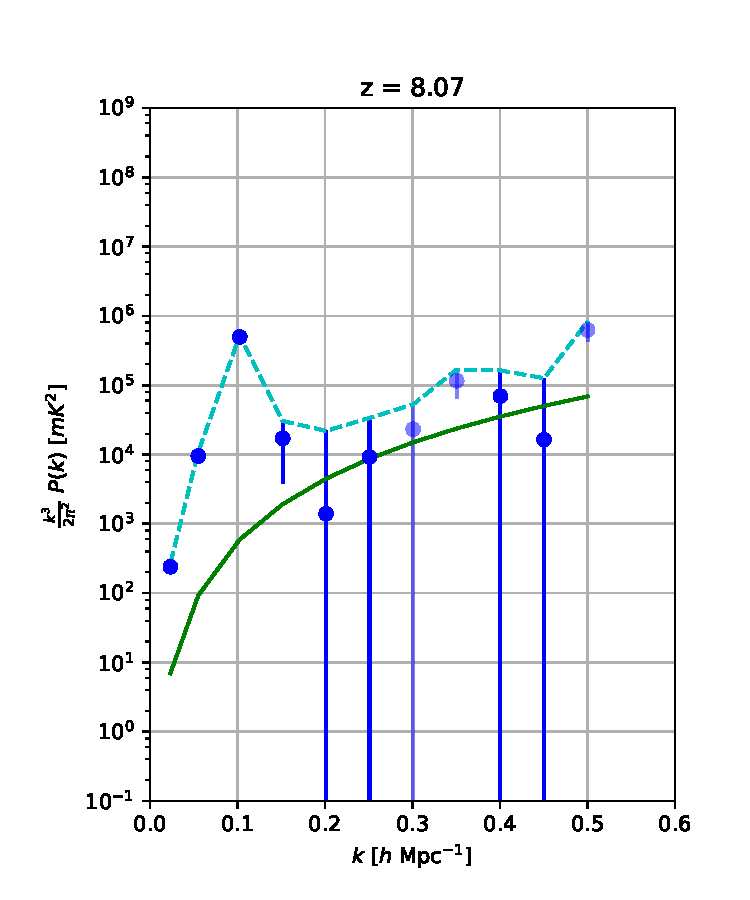
\includegraphics[scale=0.5]{chapters/psa128_pol/figures/pId_I.pdf} &
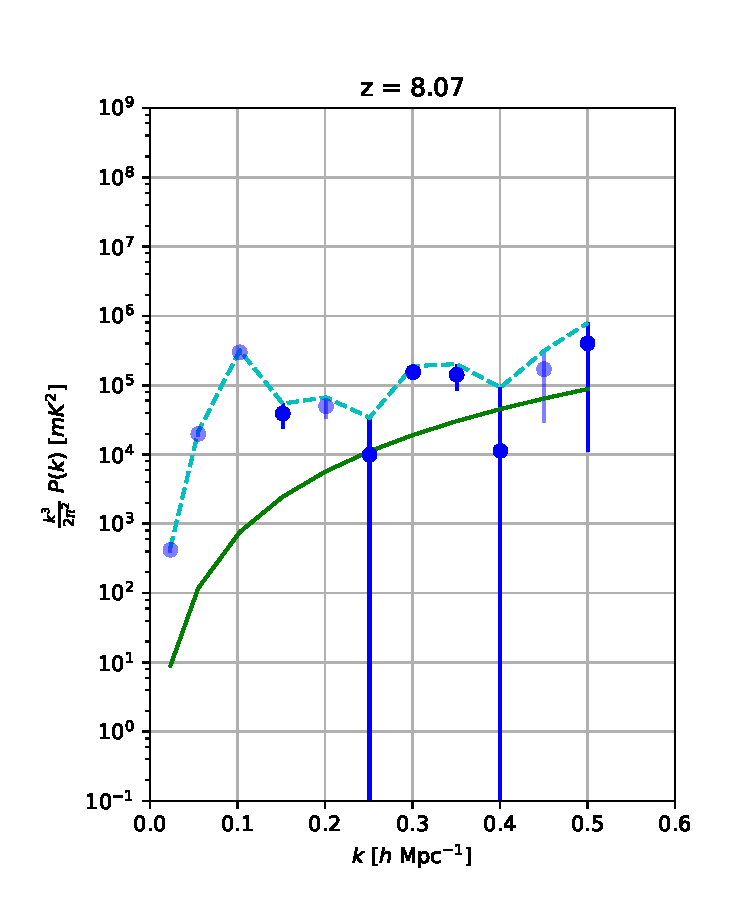
\includegraphics[scale=0.5]{chapters/psa128_pol/figures/pId_Q.pdf} \\
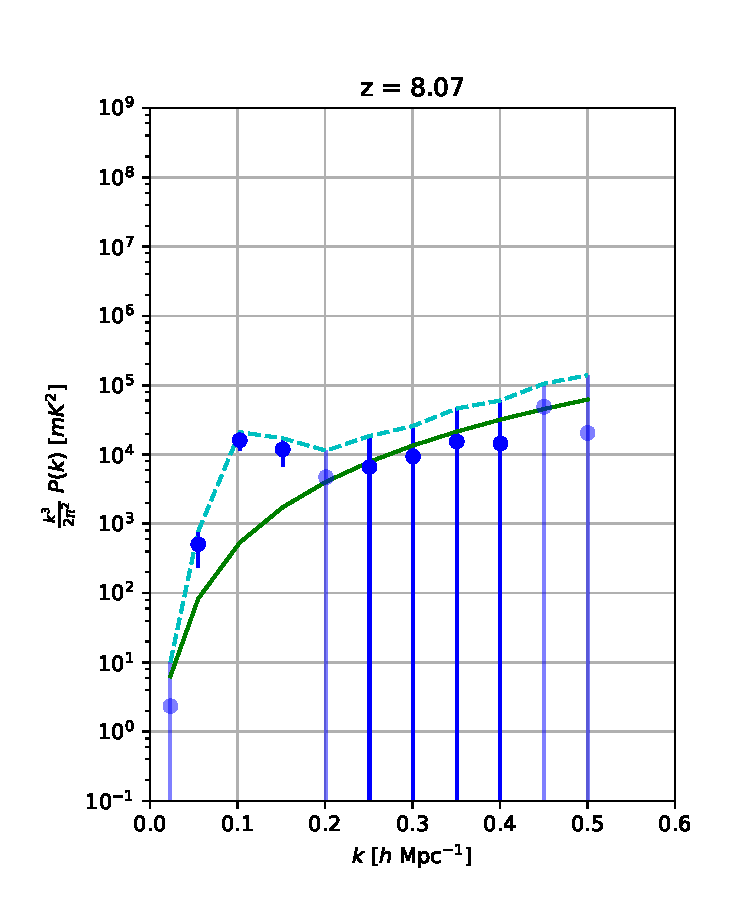
\includegraphics[scale=0.5]{chapters/psa128_pol/figures/pId_U.pdf} &
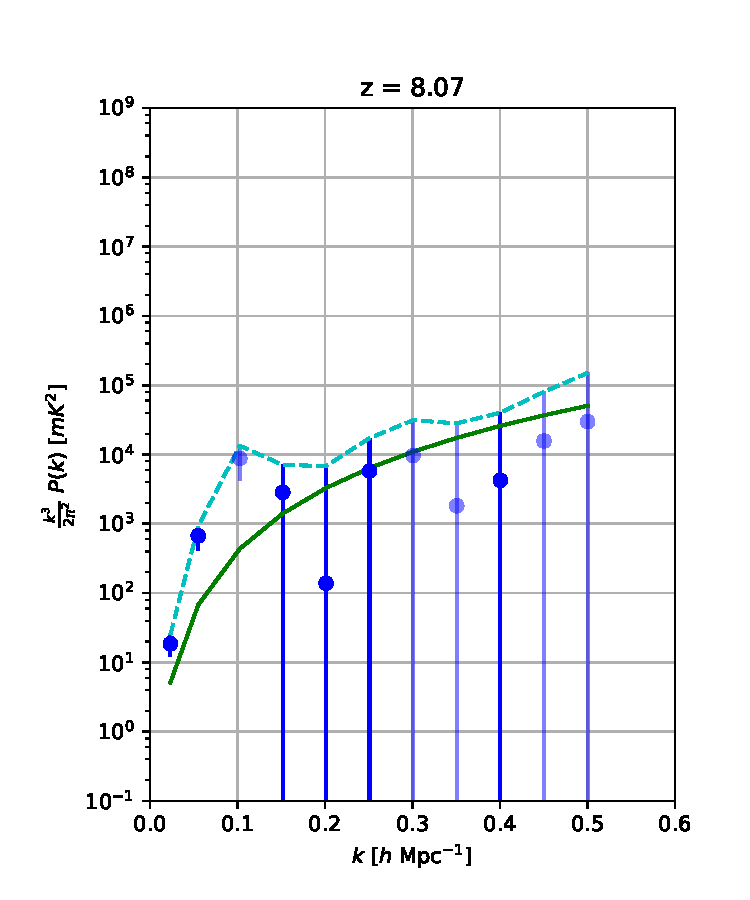
\includegraphics[scale=0.5]{chapters/psa128_pol/figures/pId_V.pdf} \\
\end{tabular}
\caption[Spherically-averaged PAPER-128 power spectra.]{Spherically-averaged power spectra in pseudo Stokes I, Q (top left, top right) U and V (bottom left, bottom right). Pale points indicate negative values. Error bars show 95\% confidence intervals, and the cyan dashed line indicates the 1$\sigma$ upper-limit given by each power spectrum. The green curve is the analytical thermal noise estimate, drawn from {\sc 21cmsense}.}
\label{fig:psa128_power_spectra_data}
\end{figure}
 
All of the power spectra in Figure~\ref{fig:psa128_power_spectra_data} showed an excess at low $k$ values, consistent with spectral structure of the PAPER beam and signal chain leaking power outside of the foreground wedge \citep{Pober.13, Kerrigan.18}. Excesses at $k\approx0.3$h/Mpc in these power spectra were also seen in PAPER-32 \citep{Moore.17} and PAPER-64 ({\color{red} Kolopanis et al. 2018}), suggesting an artefact from the PAPER signal chain was the cause.

Neglecting these artefacts, pseudo-Stokes I power spectra were broadly consistent with the analytical noise estimate, with a slight bias compared to the pure-noise power spectra of Figure~\ref{fig:psa128_power_spectra_noise}. This represented an upper limit of $\Delta^2_{\rm 21cm}(k) \lesssim (140\, {\rm mK})^2$ at $k=0.2$ h/Mpc, which is competitive with contemporary limits (e.g. {\color{red} Kolopanis et al. 2018}).

The pseudo-Stokes Q power spectrum was largely inconsistent with noise, with excesses at 0.15 h/Mpc$\leqslant\,$k$\,\leqslant$0.2 h/Mpc and 0.3 h/Mpc$\leqslant\,$k$\,\leqslant$0.35 h/Mpc. For this power to be due to Faraday-rotated emission from the diffuse foregrounds probed by a 30\,m baseline would require rotation measures of $\sim$30 rad m$^{-2}$ and $\sim$60 rad m$^{-2}$, respectively \citep{Moore.13}. Such high rotation measures have not been observed on diffuse scales \citep[e.g.][]{Oppermann.12, Bernardi.13, Lenc.16}. Neither \cite{Asad.16} nor \cite{Lenc.16} found polarized point sources of such high rotation measure in their surveys of the LOFAR and MWA EoR fields, respectively. 
\cite{Kohn.16} showed that the PAPER beam was not expected to scatter power to such high $k_{\parallel}$ values.
These factors pointed to the excess of pseudo-Stokes Q power as an indicator of calibration errors and instrument systematics leaking pseudo-Stokes I into Q. The effect is also likely larger than observed in the power spectra, as some attenuation will have occurred during LST binning due to ionospheric effects \citep[][{\color{red}; Martinot et al. (2018)}]{Moore.17}.

Simulations by \cite{Nunhokee.17} showed that Stokes Q and U power may exist at $\Delta^2_{Q,U}(k)\approx 2\times10^{4}$\,mK$^2$ levels as the ensemble average of Faraday-rotated polarized point sources (for a particularly pessimistic sky model). However, it is doubtful that we detected such power, since the pseudo-Stokes U power spectrum is so different from Q.

At $k>0.15$ h/Mpc, pseudo-Stokes U and V power spectra showed excellent consistency with noise, both in comparison the analytical noise estimate and the pure-noise power spectra shown in Figure~\ref{fig:psa128_power_spectra_noise}. This suggests that the excess in pseudo-Stokes Q, if due to calibration errors, was due to the diagonal gains being mis-matched. Uncalibrated off-diagonal gains, $D$-terms, leak pseudo-Stokes I into U and V \citep{TMS}. We saw little evidence for such leakage.

Treating power at $k=0.2$\,h/Mpc as a limit (valid for U and V, but less realistic for Q), our 1$\sigma$ upper limits on polarized power were:  $\Delta^2_{Q}(k) \lesssim (245\, {\rm mK})^2$,  $\Delta^2_{U}(k) \lesssim (100\, {\rm mK})^2$ and  $\Delta^2_{V}(k) \lesssim (83\, {\rm mK})^2$. These are the deepest limits to date on polarized power in the EoR window.

\begin{figure}
\begin{tabular}{ll}
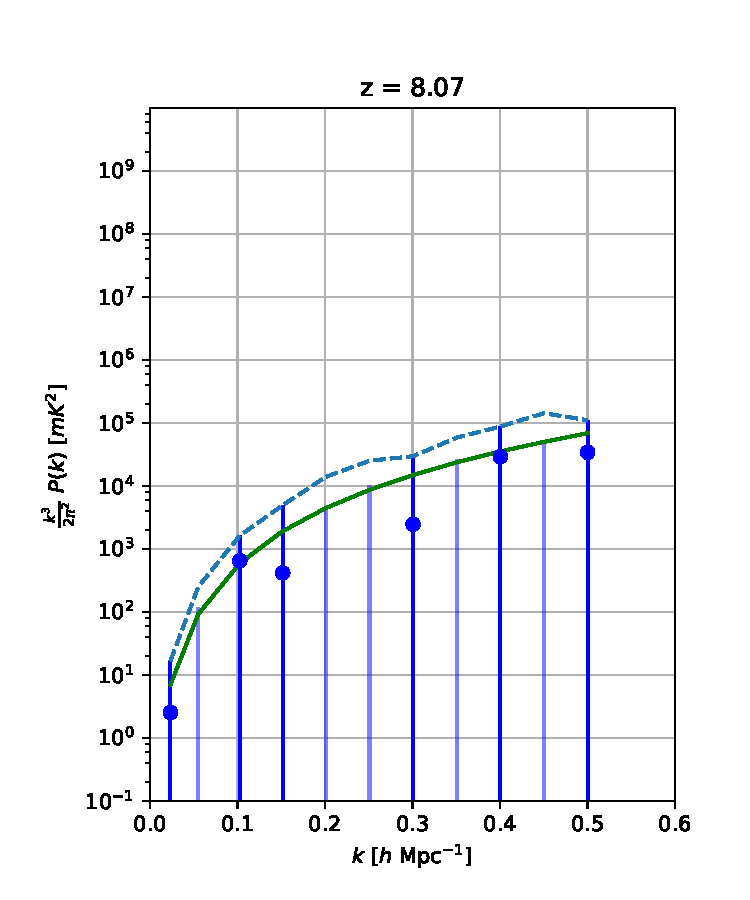
\includegraphics[scale=0.5]{chapters/psa128_pol/figures/pIn_I.pdf} &
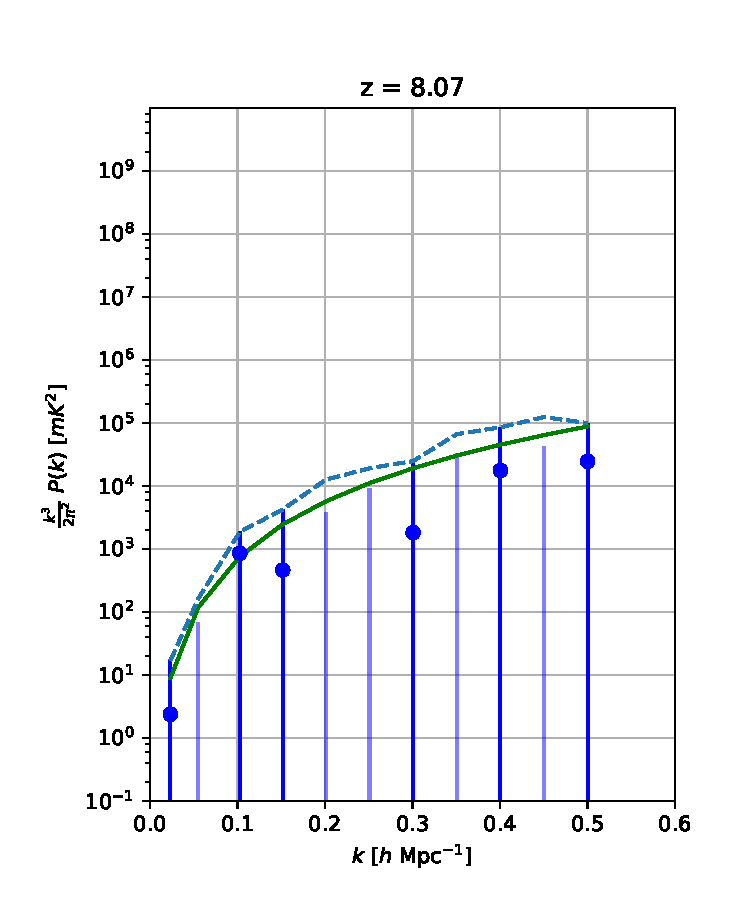
\includegraphics[scale=0.5]{chapters/psa128_pol/figures/pIn_Q.pdf} \\
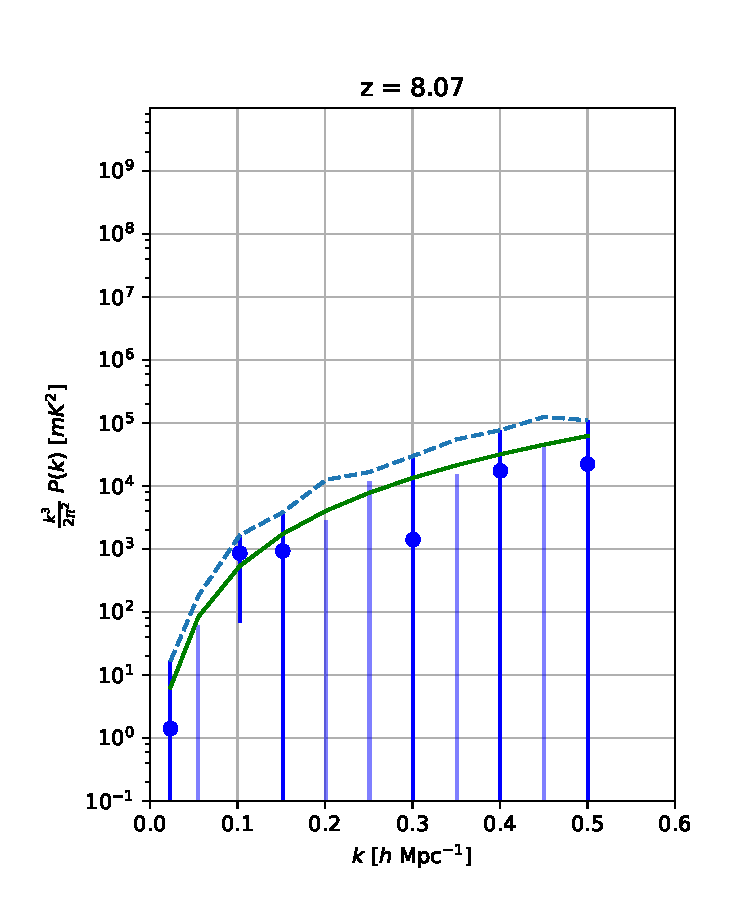
\includegraphics[scale=0.5]{chapters/psa128_pol/figures/pIn_U.pdf} &
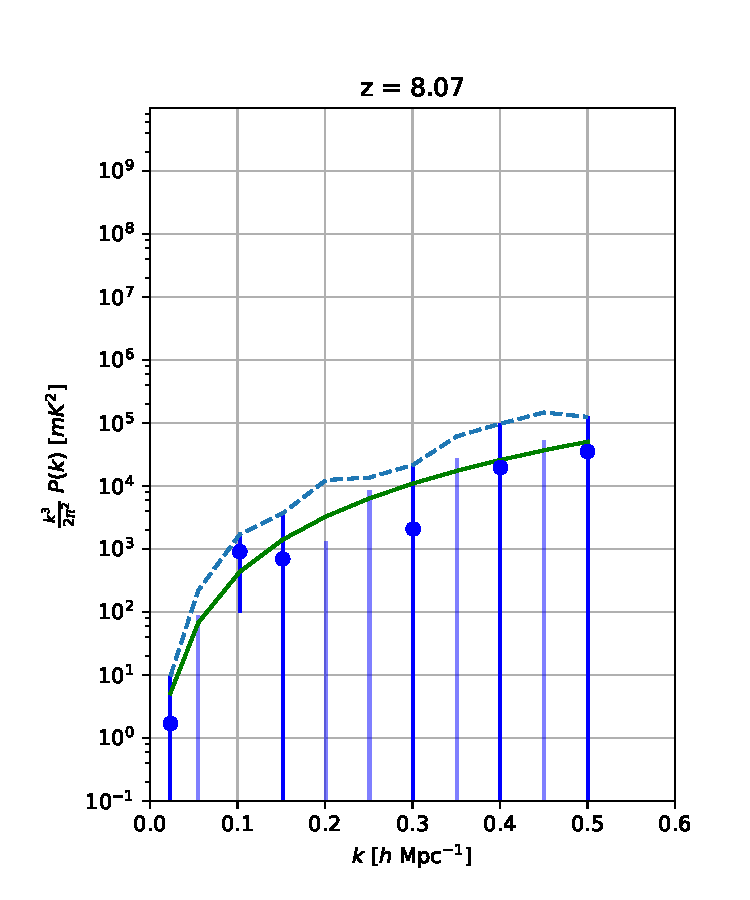
\includegraphics[scale=0.5]{chapters/psa128_pol/figures/pIn_V.pdf} \\
\end{tabular}
\caption[Spherically-averaged noise power spectra.]{Spherically-averaged power spectra of noise based on the variance of the data in our power-spectrum band. Pale points indicate negative values, error bars show 95\% confidence intervals, and the dashed line indicates the 1$\sigma$ upper-limit. All power spectrum values are consistent with the analytical noise estimate, showing the accuracy of our methods.}
\label{fig:psa128_power_spectra_noise}
\end{figure}

\section{Discussion \& Conclusions}
\label{sec:psa128_conc}

This analysis represented the first power spectrum results from PAPER-128. The processing and reduction of the two Season and seven Epochs taught us many lessons about the challenges associated with long integrations of large low-frequency arrays. These lessons were invaluable for the construction and activation of HERA, and the quality assurance techniques developed (see Chapter~\ref{chapter:data_prep_and_proc}) for such an analysis continue to be essential components of the HERA real-time system ({\color{red} Ali et al. 2018}).

\cite{Nunhokee.17} and \cite{Asad.15} predicted that the power spectrum of diffuse polarized foregrounds should exist outside of the foreground wedge at $\Delta^2(k)\approx10^3$\,mK$^2$. This is roughly two orders of magnitude above predicted EoR power \citep{Lidz.07}, and will therefore need to be extremely well characterized, since just 1\% of leakage into Stokes I could prevent an EoR detection. This study advanced that effort, setting the most stringent upper limits on pseudo-Stokes Q, U and V power to date. However, any deeper integrations with PAPER-128 may be limited by systematics due to calibration errors. 

It is unlikely that the ``detection" of power in much of the pseudo-Stokes Q power spectrum is real. However, this could be tested in the future by collecting a Epoch's-worth of ionospheric data and calculating the attenuation coefficient for different fractions of the Epoch being LST-binned together. If real pseudo-Stokes Q power is present in the power spectrum, the noise level should decrease with increasing numbers of observations in the LST bin at a rate faster than a coherent average. This variety of ``jackknifing on the ionosphere" will be investigated in future work.
